\documentclass{article}
\usepackage{graphicx} % Required for inserting images
\usepackage{listings}
\usepackage{amssymb,amsmath}
\usepackage{vmargin}
\usepackage{changepage}
\usepackage{xcolor}
\usepackage{multirow}

\definecolor{codegreen}{rgb}{0,0.6,0}
\definecolor{codegray}{rgb}{0.5,0.5,0.5}
\definecolor{codepurple}{rgb}{0.58,0,0.82}
\definecolor{backcolour}{rgb}{0.9,0.9,0.9}
\lstdefinestyle{mystyle}{
    backgroundcolor=\color{backcolour},   
    commentstyle=\color{codegreen},
    keywordstyle=\color{magenta},
    numberstyle=\tiny\color{codegray},
    stringstyle=\color{codepurple},
    basicstyle=\ttfamily\footnotesize,
    breakatwhitespace=false,         
    breaklines=true,                 
    captionpos=b,                    
    keepspaces=false,                 
    numbers=left,                    
    numbersep=5pt,                  
    showspaces=false,                
    showstringspaces=false,
    showtabs=false,                  
    tabsize=2
}
\lstset{style=mystyle}

\setpapersize{A4}
\setmargins{2.54cm}       
{2.54cm}                        
{15.92cm}                      
{23.5cm}                    
{12pt}                           
{0cm}                           
{0pt}                             
{1.5cm}
\renewcommand{\figurename}{Figura}

\renewcommand{\tablename}{Tabla}

\newcounter{codesnippet}
\newcommand{\newcodesnippet}{%
  \stepcounter{codesnippet}%
}

\title{\textbf{Proyecto del curso: El problema de la reconstrucción de cadenas}}

\author{Julian Ernesto Puyo Mora$^1$,
        Manuel Felipe Cardoso Forero$^2$,\\
        Franklin Aguirre Ortiz$^3$,
        Jean Paul Davalos Valencia$^4$\\        
        2226905$^1$, 2027288$^2$,\\
        1841743$^3$, 0000000$^4$\\
        julian.puyo@correounivalle.edu.co$^1$,\\ 
        manuel.cardoso@correounivalle.edu.co$^2$,\\
        franklin.aguirre@correounivalle.edu.co$^3$,\\
        jean.davalos@correounivalle.edu.co$^4$\\}

\date{Universidad del valle\\ Facultad de Ingeniería\\ Escuela de Ingeniería de Sistemas y Computación\\
Santiago de Cali, Diciembre 7 de 2023}

\begin{document}

\maketitle

\begin{center}
{\bf \large Resumen}\\
\end{center}

En este documento se implementarán diferentes algoritmos de multiplicación de matrices y se analizarán sus desempeños en sus versiones secuencial y paralela, y se concluirá sobre la aceleración lograda usando paralelización de tareas. También se implementarán
algoritmos para hallar el producto punto entre dos vectores, usando paralelización de
datos y se analizará su utilidad.

\section{Informe sobre funciones a implementar o usar}

Comencemos con una breve descripción sobre los tipos y valores a usar, así como de las funciones base brindadas, la cuales serán usadas en la implementación de los algoritmos propuestos.

\newcodesnippet
\begin{lstlisting}[language=Scala]
  val random = new Random()
  type Matriz = Vector[Vector[Int]]
\end{lstlisting}
\begin{center}
    \small{Fragmento de código \thecodesnippet. Definición del tipo \textit{Matriz} y del valor \textit{random}.}
\end{center}

Tal como es descrito en el fragmento de código \thecodesnippet, se define el tipo \textit{Matriz} de suma importancia ya que describe el tipo de dato \verb|Vector[Vector[Int]]|, el cual tiene ventajas sobre su indexación y es inmutable; y sobre el cual trabajaremos en nuestras funciones a desarrollar. \\

Se nos propone una función que genera \textit{Matrices} (vector bidimensional) de valores aleatorios, dado un tamaño \textit{long} y un valor \textit{vals}, el cual establece el rango \([0,vals)\) de valores para la matriz mediante el método de la clase \textit{Random}: \verb|random.nextInt(vals)|; llenando la matriz mediante el método: \verb|Vector.fill(long, long){...}|.

\newcodesnippet
\begin{lstlisting}[language=Scala]
  def matrizAlAzar(long: Int, vals: Int): Matriz = {
    // Crea una matriz de enteros cuadrada de long x long,
    // con valores aleatorios entre 0 y vals.
    val v = Vector.fill(long, long){random.nextInt(vals)}
    v
  }
\end{lstlisting}
\begin{center}
    \small{Fragmento de código \thecodesnippet. Función \textit{matrizAlAzar}.}
\end{center}

Así mismo fue propuesta la siguiente función que genera de manera similar vectores unidimensionales de tamaño: \textit{long} y rango de valores: \([0,vals)\).

\newcodesnippet
\begin{lstlisting}[language=Scala]
  def vectorAlAzar(long: Int, vals: Int): Vector[Int] = {
    //Crea un vector de enteros de longitud long,
    // con valores aleatorios entre 0 y vals
    val v = Vector.fill(long){random.nextInt(vals)}
    v
  }
\end{lstlisting}
\begin{center}
    \small{Fragmento de código \thecodesnippet. Función \textit{vectorAlAzar}.}
\end{center}

Para facilitar la implementación del algoritmo de multiplicación de matrices elemental, se propuso la función \textit{transpuesta}, la cual toma una matriz \textit{m} y retorna su transpuesta: \(m^T\). Se aprovecha el método de la clase \textit{Vector}: \textit{.tabulate} el cual genera una nueva matriz tomando como parámetro el tamaño (basado en \textit{m}): (\textit{m.length}, \textit{m.length}) y una función lambda: \verb|(i, j) => m(j)(i)|. La cual, para cada nueva posición \((i,j)\) de la matriz, coloca el elemento \((j,i)\) de \textit{m}, formando su matriz transpuesta.

\newcodesnippet
\begin{lstlisting}[language=Scala]
  def transpuesta(m: Matriz): Matriz = {
    val l = m.length
    Vector.tabulate(l, l)((i, j) => m(j)(i))
  }
\end{lstlisting}
\begin{center}
    \small{Fragmento de código \thecodesnippet. Función \textit{transpuesta}.}
\end{center}

De igual forma, fueron propuestas, tanto para la implementación de nuestras multiplicaciones matriciales en los algoritmos, como para una posterior evaluación comparativa entre una implementación de producto punto con vectores de tipo secuencial (\textit{Vector}) contra la implementación que usa su variante paralela: \textit{ParVector}.

\newcodesnippet
\begin{lstlisting}[language=Scala]
  def prodPunto(v1: Vector[Int], v2: Vector[Int]): Int = {
    (v1 zip v2).map({case (i, j) => (i*j)}).sum
  }
\end{lstlisting}
\begin{center}
    \small{Fragmento de código \thecodesnippet. Función \textit{prodPunto}.}
\end{center}

\newcodesnippet
\begin{lstlisting}[language=Scala]
  def prodPuntoParD(v1: ParVector[Int], v2: ParVector[Int]): Int = {
    // A ser usada en el punto 1.5
    (v1 zip v2).map({case (i, j) => (i*j)}).sum
  }
\end{lstlisting}
\begin{center}
    \small{Fragmento de código \thecodesnippet. Función \textit{prodPuntoParD}.}
\end{center}

Dichas funciones toman dos vectores: \textit{v1} y \textit{v2} (la primera de tipo secuencial y la segunda de tipo paralelo), y mediante los métodos \textit{.zip} y \textit{.map}, la cual multiplica los elementos de cada pareja conformada por los elementos en cada índice de \textit{v1} y \textit{v2}, creando una colección con los las diferentes parejas multiplicadas para su posterior suma mediante: \textit{.sum}. \\

Con lo anterior, podemos continuar con la descripción de las implementaciones diseñadas y desarrolladas por nosotros según el enunciado.

\subsection{Multiplicación estándar de matrices}
\subsubsection{Versión estándar secuencial}

Continuamos, con la implementación del algoritmo estándar de multiplicación de matrices; el que todos hemos usado en nuestro curso de álgebra lineal. El cual consiste, dadas dos matrices \textit{A} y \textit{B} (en nuestro caso \textit{m1} y \textit{m2}), en aplicar el producto punto entre las filas de \textit{A} con cada columna de \textit{B} formando la nueva matriz \textit{C}, tales que: \(c_{ij} = A_i \cdot B_j \). \\ 

Mediante el método: \textit{.tabulate}, de una forma similar a como fue descrito anteriormente, construye una nueva matriz de tamaño \(l \times l\) (donde \(l = m1.length\), considerando que tanto \textit{m1} como \textit{m2} tienen el mismo tamaño), donde cada elemento en la posición \((i,j)\) está dado por el producto punto entre la fila \textit{i} de \textit{m1} y la columna \textit{j} de \textit{m2}, la cual corresponde a la fila \textit{j} en la matriz transpuesta: \(m2^T\). Para lo cual se hace el llamado a la función \textit{transpuesta} con parámetro \textit{m2}.\\

\newcodesnippet
\begin{lstlisting}[language=Scala]
  def multMatriz(m1: Matriz, m2: Matriz): Matriz = {
    val m2T = transpuesta(m2)
    val l = m1.length
    val c = Vector.tabulate(l, l)((i, j) => prodPunto(m1(i),m2T(j)))
    c
  }
\end{lstlisting}
\begin{center}
    \small{Fragmento de código \thecodesnippet. Tipos a usar.}
\end{center}
\subsubsection{Versión estándar paralela}

Para nuestra versión estandar paralela, se modifica la implementación de la función anterior de tal forma en que, mediante la función \textit{parallel} se ejecutan en simultáneo el llamado a la operación \(transpuesta(m2)\) y el cálculo de \textit{m1.length}. Así como la ejecución del método \textit{.tabulate} de tal forma en que sea llevado a cabo en dos tareas. Para ello se introdujo un nuevo valor llamado \textit{middle} el cual registra la mitad truncada de \(l = m1.length\), según el cual se divide la ejecución de \textit{.tabulate} en dos tareas según éste sea par o impar, ya que el fín es que la primera tarea ejecute la primera parte de la matriz \(C_{ij}\), tales que \(0 \leq i \leq middle\) cuando \textit{middle} es par, o \(0 \leq i \leq middle + 1\) cuando es impar. Así la segunda tarea se encargará de calcular el resto de filas de la matriz \(C_{ij}\), tales que \(middle \leq i < l\) cuando \textit{middle} es par, o \(middle + 1 \leq i < l\) cuando es impar. Aprovechando el funcionamiento de \textit{.tabulate}, el cual itera sobre la función anónima entregada, comenzando desde los valores \((i,j) = (0,0)\), y entregando, tal como fue ya descrito, una matriz de tamaño \(l \times l\). Por lo que modificando dicho tamaño o dichos valores de \textit{i} o \textit{j} dentro de la función anónima, se consigue dividir el rango deseado para las filas a construir dentro de cada tarea. Su correctitud será estudiada en la siguiente sección.\\

\newcodesnippet
\begin{lstlisting}[language=Scala]
  def multMatrizPar(m1: Matriz, m2: Matriz): Matriz = {
    val (m2T:Matriz,l:Int) = parallel(transpuesta(m2),m1.length)
    val middle = l/2
    val (c1:Matriz, c2:Matriz) = {
      if (l % 2 == 0)
        parallel(
          Vector.tabulate(middle, l)((i, j) => prodPunto(m1(i), m2T(j))),
          Vector.tabulate(middle, l)((i, j) => prodPunto(m1(i + middle), m2T(j)))
        )
      else
        parallel(
          Vector.tabulate(middle + 1, l)((i, j) => prodPunto(m1(i), m2T(j))),
          Vector.tabulate(middle, l)((i, j) => prodPunto(m1(i + middle + 1), m2T(j)))
        )
    }
    val c = c1++c2
    c
  }
\end{lstlisting}
\begin{center}
    \small{Fragmento de código \thecodesnippet. Tipos a usar.}
\end{center}
\subsection{Multiplicación recursiva de matrices}

Para la implementación de un algoritmo recursivo, con el enfoque de \textit{"dividir y conquitar"}, serán necesarias dos funciones auxiliares: \textit{subMatriz} y \textit{sumMatriz}. Bajo el esquema del algoritmo propuesto en el enunciado ilustrado por:

\begin{figure}[h]
    \begin{minipage}{1\textwidth}
        \centering
        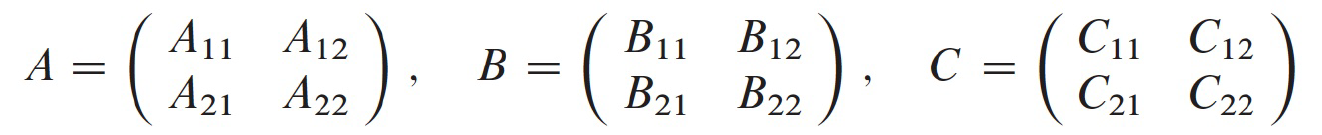
\includegraphics[scale=0.3]{Imagen1.png}
        \caption{Matrices \textit{A}, \textit{B} y \textit{C} expresadas en submatrices.}
        \label{1}
    \end{minipage}
\end{figure}

\begin{figure}[h]
    \begin{minipage}{1\textwidth}
        \centering
        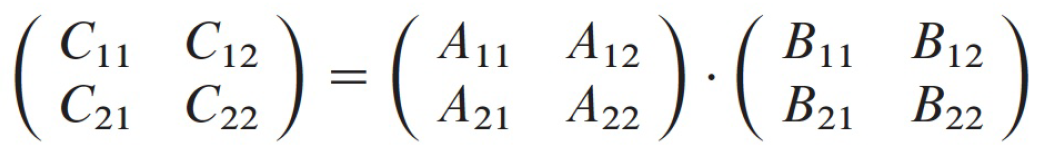
\includegraphics[scale=0.25]{Imagen2.png}
        \caption{Equivalencia de \textit{C} en términos de \textit{A} y \textit{B}.}
        \label{1}
    \end{minipage}
\end{figure}


Donde el objetivo será dividir la matrices recibidas en cada recursión en cuatro submatrices y para éstas realizar las operaciones que nos darán las cuatros submatrices que conformarán la matriz deseada \textit{C} tales que:

\begin{figure}[h]
    \begin{minipage}{1\textwidth}
        \centering
        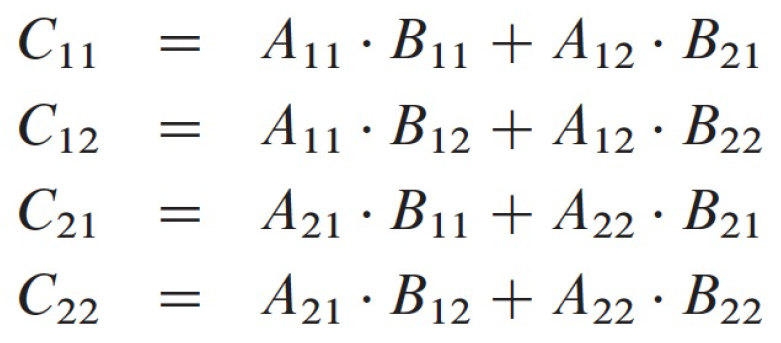
\includegraphics[scale=0.25]{Imagen3.png}
        \caption{Equivalencia de las submatrices de \textit{C} en términos de las submatrices de \textit{A} y \textit{B}.}
        \label{1}
    \end{minipage}
\end{figure}

\subsubsection{Extrayendo submatrices}

En la implementación de la función propuesta \textit{subMatriz} encontramos que recibe como parámetros la matriz \textit{m}, los valores \textit{i} y \textit{j}, (correspondientes a los índices de la posición \((i,j)\), desde la cual se comenzará a construir la submatriz a retornar) y el valor \textit{l} el cual dictará el tamaño de la submatriz a retornar. 

\newcodesnippet
\begin{lstlisting}[language=Scala]
  def subMatriz(m: Matriz, i: Int, j: Int, l: Int): Matriz = {
    // Dada m, matriz cuadrada de NxN, 1<=i , j<=N, i+n<=N, j+n<=N,
    // devuelve la submatriz de nxn correspondiente a m[i..i+(n-1), j..j+(n-1)]
    val posI = i
    val posJ = j
    Vector.tabulate(l,l)((i,j) => m(i+posI)(j+posJ))
  }
\end{lstlisting}
\begin{center}
    \small{Fragmento de código \thecodesnippet. Función \textit{subMatriz}.}
\end{center}

Con lo cual, se puede identificar en el código que, dentro del llamado a \textit{.tabulate} se construye la submatriz de tamaño \(l \times l\) desde la posición \((posI, posJ)\) (tales que \(posI = i\) y \(posJ = j\), \textit{i} y \textit{j} recibidos como parámetro), con valores: \(m(i + posI)(j + posJ)\) en cada posición \((i,j)\) de la submatriz, marcando el punto de inicio deseado. Se debe tener en cuenta que existen ciertas condiciones para los valores de \textit{i}, \textit{j} y \textit{l}. Los cuales deben obedecer que las submatrices solicitadas deben estar, de hecho, dentro de \textit{m}.

\subsubsection{Sumando matrices}

En el mismo sentido expresado en el uso del método \textit{.tabulate} pero cambiando la función anónima a utilizar se implementó la función \textit{sumMatriz}, cuyo objetivo es, dadas las matrices \textit{m1} y \textit{m2}, formar una nueva matriz \textit{m}, tales que cada elemento \(m_{ij}\) es está formado por \(m1_{ij} + m2_{ij}\). Lo cual se puede identificar en la línea 6 del fragmento de código ilustrado a continuación.\\

\newcodesnippet
\begin{lstlisting}[language=Scala]
  def sumMatriz(m1: Matriz, m2: Matriz): Matriz = {
    // recibe m1 y m2 matrices cuadradas de la misma dimension, potencia de 2
    // y de vuelve la matriz resultante de la suma de las 2 matrices
    val l = m1.length
    Vector.tabulate(l,l)((i,j) => m1(i)(j)+m2(i)(j))
  }
\end{lstlisting}
\begin{center}
    \small{Fragmento de código \thecodesnippet. Función \textit{sumMatriz}.}
\end{center}
\subsubsection{Multiplicando matrices recursivamente, versión secuencial}

Ahora, con las funciones \textit{sumMatriz} y \textit{subMatriz} implementadas, desarrollamos e implementamos el algoritmo propuesto (figura 3), claramente con el objetivo implícito de hacer recursión con las submatrices respectivas hasta llegar a un valor de \(l = 2\) en cada submatriz, siendo ésta la condición de parada donde será llamada a nuestra función \textit{multMatriz}, la cual se espera que opere matrices de tamaño 2. Dicha función fue usada en vez de aplicar de nuevo \textit{Vector.tabulate} con el fin de ahorrar código.\\

Entonces, el objetivo de \textit{multMatrizRec} es el de devolver la multiplicación de \textit{m1} y \textit{m2}, mediante el algoritmo descrito para la cada recursión: En cada llamado a la función se realiza una división en submatrices de las matrices recibidas como parámetros, para luego ser operadas según lo propuesto en las figuras: 1, 2 y 3. Su correctitud será discutida en la sección 2.

\newcodesnippet
\begin{lstlisting}[language=Scala]
  def multMatrizRec(m1: Matriz, m2: Matriz): Matriz = {
    // recibe m1 y m2 matrices cuadradas de la misma dimension, potencia de 2
    // y devuelve la multiplicacion de las 2 matrices
    val l = m1.length
    val mid = l/2
    if (l == 2 || l == 1) {
      multMatriz(m1,m2)
    }
    else {
      val c_00 = sumMatriz(
        multMatrizRec(
          subMatriz(m1, 0, 0, mid),
          subMatriz(m2, 0, 0, mid)),
        multMatrizRec(
          subMatriz(m1, 0, mid, mid),
          subMatriz(m2, mid, 0, mid))
      )
      val c_0mid = sumMatriz(
        multMatrizRec(
          subMatriz(m1, 0, 0, mid),
          subMatriz(m2, 0, mid, mid)),
        multMatrizRec(
          subMatriz(m1, 0, mid, mid),
          subMatriz(m2, mid, mid, mid))
      )
      val c_mid0 = sumMatriz(
        multMatrizRec(
          subMatriz(m1, mid, 0, mid),
          subMatriz(m2, 0, 0, mid)),
        multMatrizRec(
          subMatriz(m1, mid, mid, mid),
          subMatriz(m2, mid, 0, mid))
      )
      val c_midmid = sumMatriz(
        multMatrizRec(
          subMatriz(m1, mid, 0, mid),
          subMatriz(m2, 0, mid, mid)),
        multMatrizRec(
          subMatriz(m1, mid, mid, mid),
          subMatriz(m2, mid, mid, mid))
      )
      (c_00 ++ c_mid0).zip(c_0mid ++ c_midmid).map {case (row1, row2) => row1 ++ row2}
    }
  }
\end{lstlisting}
\begin{center}
    \small{Fragmento de código \thecodesnippet. Función \textit{multMatrizRec}.}
\end{center}

Nótese que se hizo uso de un valor igual al truncamiento de la división \(l/2\), donde \(l = m1.length\). Dicho valor es clave. Ya que, al examinar el algoritmo a usar, notamos que cada matriz se divide en submatrices en una de proporción 1:4, donde cada matriz es de igual tamaño (tamaño igual a \(l/2 \times l/2 \)). Por lo que hallar \textit{mid} es de suma importancia, ya que será el que demarcará el tamaño de cada submatriz así como la posición desde donde cada una será construida. \\

En resumen, en cada llamado a \textit{multMatrizRec}, cuando \(l > 2\), se hallarán las submatrices de \textit{C} mediante las operaciones \textit{sumMatriz} y su llamado recursivo, pero ahora con las submatrices de \textit{m1} y de \textit{m2} halladas con \textit{subMatriz} (véase: Figura 3). Donde seguirá habiendo recursividad hasta que las submatrices dadas sean de tamaño \(2 \times 2\). Los valores de \textit{C} son \(c_{00}\), \(c_{0mid}\), \(c_{mid0}\) y \(c_{midmid}\), que describen las submatrices que comienzan en \((0,0)\), \((0,mid)\), \((mid,0)\) y \((mid,mid)\) respectivamente. Dichas submatrices en cada recursión son unidas mediante: \verb|(c_00 ++ c_mid0).zip(c_0mid ++ c_midmid).map {| \verb|case (row1, row2) => row1 ++ row2}|. Función la cual une las las columnas de \verb|c_00 ++ c_mid0| con las de \verb|c_0mid ++ c_midmid| por fila.

\subsubsection{Multiplicando matrices recursivamente, versión paralela}

En su versión paralela, se buscó que las operaciones recursivas realizadas ocurrieran en tareas separadas por \textit{task} y ubicadas en tuplas, para luego ser llamados sus valores en las evaluaciones que determinarían los valores de \textit{C}. Con ello logrando paralelismo dentro de cada una de ellas. Pudo haberse estudiado el uso de \textit{parallel} para realizar todas las tareas en simultáneo, sin embargo, se optó por el uso de \textit{task}, al igual que para todas las implementaciones en paralelo encontradas en este taller.\\

Luego se estudiarán los resultados sobre qué tanto mejora el tiempo de ejecución y oportunidades de optimización. \\

\newcodesnippet
\begin{lstlisting}[language=Scala]
  def multMatrizRecPar(m1: Matriz, m2: Matriz): Matriz = {
    // recibe m1 y m2 matrices cuadradas de la misma dimension, potencia de 2
    // y devuelve la multiplicacion de las 2 matrices
    val l = m1.length
    val mid = l / 2

    val umbral = 4
    val threshold = {
      if (l <= umbral)
        l
      else
        umbral
    }

    if (l == threshold) { // 'threshold' define si se usa el algoritmo secuencial o paralelo.
      multMatrizRec(m1, m2)
    }
    else {
      val (t1, t2) = (
        task(multMatrizRecPar(
          subMatriz(m1, 0, 0, mid),
          subMatriz(m2, 0, 0, mid))),
        task(multMatrizRecPar(
          subMatriz(m1, 0, mid, mid),
          subMatriz(m2, mid, 0, mid)))
      )
      val (t3, t4) = (
        task(multMatrizRecPar(
          subMatriz(m1, 0, 0, mid),
          subMatriz(m2, 0, mid, mid))),
        task(multMatrizRecPar(
          subMatriz(m1, 0, mid, mid),
          subMatriz(m2, mid, mid, mid)))
      )
      val (t5, t6) = (
        task(multMatrizRecPar(
          subMatriz(m1, mid, 0, mid),
          subMatriz(m2, 0, 0, mid))),
        task(multMatrizRecPar(
          subMatriz(m1, mid, mid, mid),
          subMatriz(m2, mid, 0, mid)))
      )
      val (t7, t8) = (
        task(multMatrizRecPar(
          subMatriz(m1, mid, 0, mid),
          subMatriz(m2, 0, mid, mid))),
        task(multMatrizRecPar(
          subMatriz(m1, mid, mid, mid),
          subMatriz(m2, mid, mid, mid)))
      )

      val (m1_00_m2_00, m1_0mid_m2_mid0) = (t1.join, t2.join)
      val (m1_00_m2_0mid, m1_0mid_m2_midmid) = (t3.join, t4.join)
      val (m1_mid0_m2_00, m1_midmid_m2_mid0) = (t5.join, t6.join)
      val (m1_mid0_m2_0mid, m1_midmid_m2_midmid) = (t7.join, t8.join)

      val c_00 = sumMatriz(m1_00_m2_00, m1_0mid_m2_mid0)
      val c_0mid = sumMatriz(m1_00_m2_0mid, m1_0mid_m2_midmid)
      val c_mid0 = sumMatriz(m1_mid0_m2_00, m1_midmid_m2_mid0)
      val c_midmid = sumMatriz(m1_mid0_m2_0mid, m1_midmid_m2_midmid)
      (c_00 ++ c_mid0).zip(c_0mid ++ c_midmid).map {case (row1, row2) => row1 ++ row2}
    }
  }
\end{lstlisting}
\begin{center}
    \small{Fragmento de código \thecodesnippet. Función \textit{multMatrizRecPar}.}
\end{center}

Cabe resaltar que también fue de importancia agregar en el diseño y desarrollo, la posibilidad de aplicar un umbral que determine desde qué punto se ejecute la versión secuencial en vez de la paralela; y de que éste sea modificable. El objetivo de dicho umbral sería el de optimizar la ejecución de las versiones paralelas (sería diseñado de igual forma para la implementación paralelas del algoritmo de Strassen), para que, cuando sea poco óptimo ejecutar la función paralela, comparando con la secuencial, en tamaños de matriz mayores que 2 (no haya \textit{speedup}), pueda hacerse el llamado a la función secuencial, dentro de la recursión. Lo dicho será estudiado y descrito a fondo en su sección respectiva, así mismo se explicará la decisión de haber tomado el umbral igual a 4. 

\subsection{Multiplicación de matrices usando el algoritmo de Strassen}

Para la implementación del algoritmo de Strassen se parte de la misma idea de hacer recursión, pero disminuyendo la cantidad de multiplicaciones recursivas necesarias, buscando un tiempo de ejecución menor, en comparación con el algoritmo anterior. En efecto se dice que es el algoritmo más óptimo para la multiplicación de matrices. Lo cual se pondrá a prueba en nuestro Análisis Comparativo encontrado en la última sección. Dicho algoritmo comprende las siguientes operaciones, las cuales serán replicadas en nuestra implementación:

\begin{figure}[h]
    \begin{minipage}{1\textwidth}
        \centering
        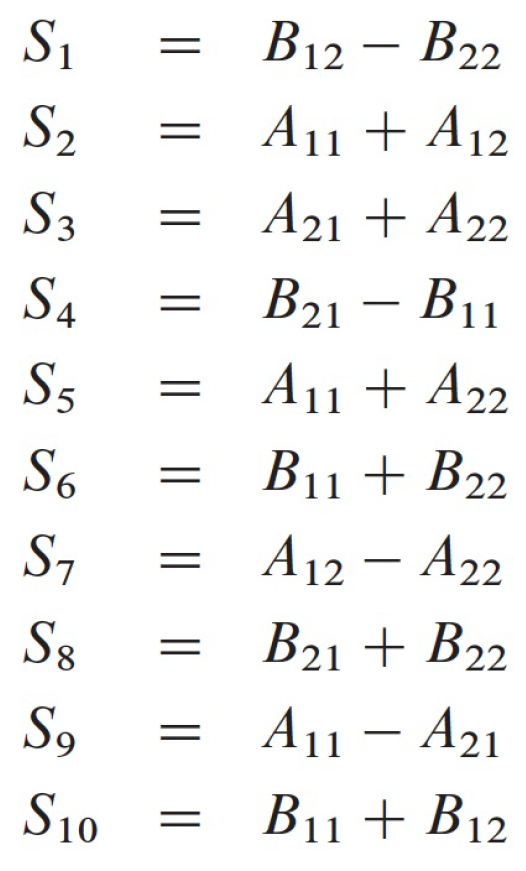
\includegraphics[scale=0.25]{Imagen4.png}
        \caption{Valores de \textit{S} en términos de \textit{A} y \textit{B}.}
        \label{1}
    \end{minipage}
\end{figure}

Como se puede notar, será requerida la implementación de una función que nos permita restar matrices, para hallar los valores de \textit{S}.\\

Así mismo será necesario hacer operaciones de multiplicación de matrices, tomando los valores de \textit{S} encontrados y operarlos, ya sea entre sí mismos o con submatrices de \textit{A} y de \textit{B}, tal como se puede ver a continuación.

\begin{figure}[h]
    \begin{minipage}{1\textwidth}
        \centering
        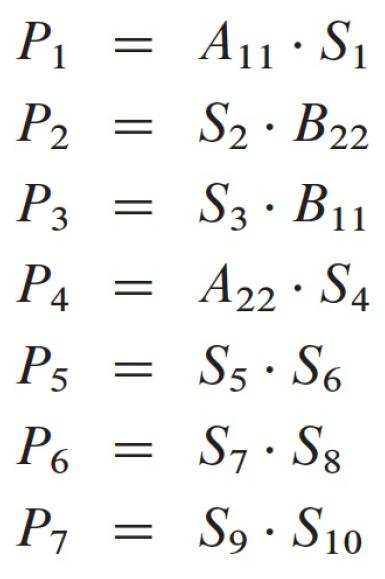
\includegraphics[scale=0.25]{Imagen5.png}
        \caption{Valores de \textit{P} en términos de \textit{A} y \textit{B}.}
        \label{1}
    \end{minipage}
\end{figure}

\begin{figure}[h]
    \begin{minipage}{1\textwidth}
        \centering
        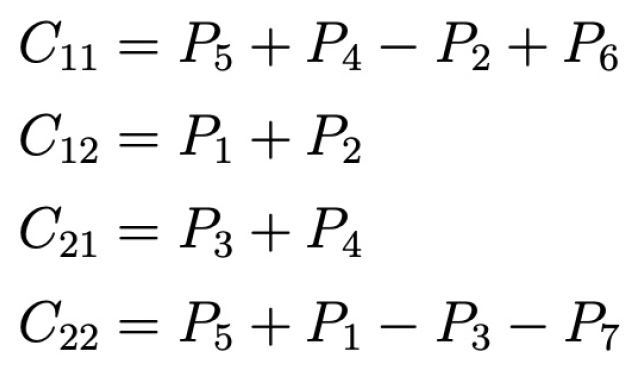
\includegraphics[scale=0.25]{Imagen6.png}
        \caption{Equivalencia de las submatrices de \textit{C} en términos de \textit{P}.}
        \label{1}
    \end{minipage}
\end{figure}

\subsubsection{Restando matrices}

Nuestra función \textit{restaMatriz} fue desarrollada bajo el mismo diseño de \textit{sumMatriz} cambiando el operador dentro del lado derecho de la función lambda \verb|(i,j) => m1(i)(j)-m2(i)(j)| encontrada como parámetro dentro de \verb|Vector.tabulate(l,l)(...)|, el cual es un operador resta. Logrando así el objetivo de retornar la matriz \textit{m} de tamaño \textit{l}, tal que \(m = m1_{ij} - m2_{ij}\).

\newcodesnippet
\begin{lstlisting}[language=Scala]
  def restaMatriz(m1: Matriz, m2: Matriz): Matriz = {
    // recibe m1 y m2 matrices cuadradas de la misma dimension, potencia de 2
    // y devuelve la matriz resultante de la resta de las 2 matrices
    val l = m1.length
    Vector.tabulate(l,l)((i,j) => m1(i)(j)-m2(i)(j))
  }
\end{lstlisting}
\begin{center}
    \small{Fragmento de código \thecodesnippet. Función \textit{restaMatriz}.}
\end{center}
\subsubsection{Algoritmo de Strassen, versión secuencial}

Con la función \textit{restaMatriz} implementada desarrollamos la función \textit{multStrassen}, la cual ejecuta dentro de su llamado, cuando no se cumple la condición de parada, la multiplicación de matrices mediante recursión, ejecutando en cada una de ellas lo ilustrado en las figuras 4 y 5, para hallar los valores de \textit{S} y \textit{P}, con el fin de obtener las 4 submatrices de \textit{C}, según es ilustrado en la figura 6. \\

La implementación se desarrolló en tuplas con el fin de simplificar la modificación y desarrollo posterior de \textit{multStrassenPar} mediante el uso de la función \textit{parallel} en cada una de ellas. Sin embargo al final se optó por una implementación mediante la abstracción \textit{task} y \textit{join}.

\newcodesnippet
\begin{lstlisting}[language=Scala]
  def multStrassen(m1: Matriz, m2: Matriz): Matriz = {
    // recibe m1 y m2 matrices cuadradas de la misma dimension, potencia de 2
    // y devuelve la multiplicacion de las 2 matrices usando el algoritmo de Strassen
    val l = m1.length
    val mid = l / 2
    if (l == 2 || l == 1) {
      multMatriz(m1, m2)
    }
    else {
      val (s1, s2) = (
        restaMatriz(
          subMatriz(m2, 0, mid, mid),
          subMatriz(m2, mid, mid, mid)),
        sumMatriz(
          subMatriz(m1, 0, 0, mid),
          subMatriz(m1, 0, mid, mid))
      )
      val (s3, s4) = (
        sumMatriz(
          subMatriz(m1, mid, 0, mid),
          subMatriz(m1, mid, mid, mid)),
        restaMatriz(
          subMatriz(
            m2, mid, 0, mid),
          subMatriz(m2, 0, 0, mid))
      )
      val (s5, s6) = (
        sumMatriz(
          subMatriz(m1, 0, 0, mid),
          subMatriz(m1, mid, mid, mid)),
        sumMatriz(
          subMatriz(m2, 0, 0, mid),
          subMatriz(m2, mid, mid, mid))
      )
      val (s7, s8) = (
        restaMatriz(
          subMatriz(m1, 0, mid, mid),
          subMatriz(m1, mid, mid, mid)),
        sumMatriz(
          subMatriz(m2, mid, 0, mid),
          subMatriz(m2, mid, mid, mid))
      )
      val (s9, s10) = (
        restaMatriz(
          subMatriz(m1, 0, 0, mid),
          subMatriz(m1, mid, 0, mid)),
        sumMatriz(
          subMatriz(m2, 0, 0, mid),
          subMatriz(m2, 0, mid, mid))
      )

      val (p1, p2) = (
        multStrassen(subMatriz(m1, 0, 0, mid), s1),
        multStrassen(s2, subMatriz(m2, mid, mid, mid))
      )
      val (p3, p4) = (
        multStrassen(s3, subMatriz(m2, 0, 0, mid)),
        multStrassen(subMatriz(m1, mid, mid, mid), s4)
      )
      val (p5, p6) = (
        multStrassen(s5, s6),
        multStrassen(s7, s8)
      )
      val p7 = multStrassen(s9, s10)

      val c_00 = sumMatriz(restaMatriz(sumMatriz(p5, p4), p2), p6)
      val c_0mid = sumMatriz(p1, p2)
      val c_mid0 = sumMatriz(p3, p4)
      val c_midmid = restaMatriz(restaMatriz(sumMatriz(p5, p1), p3), p7)
      (c_00 ++ c_mid0).zip(c_0mid ++ c_midmid).map { case (row1, row2) => row1 ++ row2 }
    }
  }
\end{lstlisting}
\begin{center}
    \small{Fragmento de código \thecodesnippet. Función \textit{multStrassen}.}
\end{center}
\subsubsection{Algoritmo de Strassen, versión paralela}

Tal como fue enunciado anteriormente, la implementación de \textit{multStrassenPar} comprende unas pocas modificaciones sobre \textit{multStrassen}(), que se resumen en: la configuración de un umbral modificable, la integración de la función \textit{task} y \textit{join} sobre los valores en las tuplas definidas y el llamado recursivo a \textit{multStrassenPar}(), en lugar de \textit{multStrassen}(). Así mismo, cuando se cumpla la condición de parada (definido por el \textit{umbral}) se hará el llamado a la función secuencial, en vez de \textit{multMatriz}().

\newcodesnippet
\begin{lstlisting}[language=Scala]
  def multStrassenPar(m1: Matriz, m2: Matriz): Matriz = {
    // recibe m1 y m2 matrices cuadradas de la misma dimension, potencia de 2
    // y devuelve la multiplicacion de las 2 matrices usando el algoritmo de Strassen
    val l = m1.length
    val mid = l / 2

    val umbral = 4
    val threshold = {
      if (l <= umbral)
        l
      else
        umbral
    }

    if (l == threshold) {
      multStrassen(m1, m2)
    }
    else {
      val (t1, t2) = (
        task(restaMatriz(
          subMatriz(m2, 0, mid, mid),
          subMatriz(m2, mid, mid, mid))),
        task(sumMatriz(
          subMatriz(m1, 0, 0, mid),
          subMatriz(m1, 0, mid, mid)))
      )
      val (t3, t4) = (
        task(sumMatriz(
          subMatriz(m1, mid, 0, mid),
          subMatriz(m1, mid, mid, mid))),
        task(restaMatriz(
          subMatriz(m2, mid, 0, mid),
          subMatriz(m2, 0, 0, mid)))
      )
      val (t5, t6) = (
        task(sumMatriz(
          subMatriz(m1, 0, 0, mid),
          subMatriz(m1, mid, mid, mid))),
        task(sumMatriz(
          subMatriz(m2, 0, 0, mid),
          subMatriz(m2, mid, mid, mid)))
      )
      val (t7, t8) = (
        task(restaMatriz(
          subMatriz(m1, 0, mid, mid),
          subMatriz(m1, mid, mid, mid))),
        task(sumMatriz(
          subMatriz(m2, mid, 0, mid),
          subMatriz(m2, mid, mid, mid)))
      )
      val (t9, t10) = (
        task(restaMatriz(
          subMatriz(m1, 0, 0, mid),
          subMatriz(m1, mid, 0, mid))),
        task(sumMatriz(
          subMatriz(m2, 0, 0, mid),
          subMatriz(m2, 0, mid, mid)))
      )

      val (s1, s2) = (t1.join, t2.join)
      val (s3, s4) = (t3.join, t4.join)
      val (s5, s6) = (t5.join,t6.join)
      val (s7, s8) = (t7.join, t8.join)
      val (s9, s10) = (t9.join, t10.join)


      val (t11, t12) = (
        task(multStrassenPar(subMatriz(m1, 0, 0, mid), s1)),
        task(multStrassenPar(s2, subMatriz(m2, mid, mid, mid)))
      )
      val (t13, t14) = (
        task(multStrassenPar(s3, subMatriz(m2, 0, 0, mid))),
        task(multStrassenPar(subMatriz(m1, mid, mid, mid), s4))
      )
      val (t15, t16) = (
        task(multStrassenPar(s5, s6)),
        task(multStrassenPar(s7, s8))
      )
      val t17 = task(multStrassenPar(s9, s10))

      val (p1, p2) = (t11.join, t12.join)
      val (p3, p4) = (t13.join, t14.join)
      val (p5, p6) = (t15.join, t16.join)
      val p7 = t17.join

      val c_00 = sumMatriz(restaMatriz(sumMatriz(p5, p4), p2), p6)
      val c_0mid = sumMatriz(p1, p2)
      val c_mid0 = sumMatriz(p3, p4)
      val c_midmid = restaMatriz(restaMatriz(sumMatriz(p5, p1), p3), p7)
      (c_00 ++ c_mid0).zip(c_0mid ++ c_midmid).map {case (row1, row2) => row1 ++ row2}
    }
  }
\end{lstlisting}
\begin{center}
    \small{Fragmento de código \thecodesnippet. Función \textit{multStrassenPar}.}
\end{center}

\section{Informe de corrección}

A continuación se encontrarán las argumentaciones acerca de la correctitud de las funciones implementadas.

\subsection{Multiplicación estándar de matrices}
\subsubsection{Versión estándar secuencial}
\textbf{Argumentación sobre la corrección}\\

Para demostrar la correctitud de la función implementada \textit{multMatriz}, sea \(P_f\) tal que \(P_f == multMatriz()\), y sea \textit{f} la función que retorna los valores esperados \textit{m} (recordemos el algoritmo estandar de multiplicación de matrices), dadas las matrices \textit{m1} y \textit{m2} de valores y tamaño cualesquiera.\\

Deseamos probar que:

\begin{equation*}
    P_f \equiv f = m
\end{equation*}

Tal que \textit{m} es la matriz de elementos \(m_{ij} = m1_{i} \cdot m2^T_{j}\), donde \(m1_{i}\) es la fila \textit{i} de \textit{m1} y \(m2^T_{j}\) es la columna \textit{j} de \textit{m2}.\\

Evaluemos mediante el modelo de sustitución:

\begin{align*}
    &multMatriz(m1, m2)\\
    &\rightarrow val \ m2T = transpuesta(m2)\\
    &\quad \; \; val \ l = m1.length\\
    &\rightarrow val \ c = Vector.tabulate(l, l)((i, j) => prodPunto(m1(i),m2T(j)))\\
    &\rightarrow c\\
    &\equiv m\\
\end{align*}

Por lo tanto: 

\begin{equation*}
    P_f \equiv f = m
\end{equation*}

Lo cual se cumple considerando como verdadera la correctitud de las funciones: \(Vector.tabulate()()\) y \(prodPunto()\). Recuérdese, tal como fue descrito en la sección anterior, el funcionamiento de \textit{.tabulate}, el cual construye una matriz de tamaño \(l \times l\), con valores: \((i,j), 0 \leq i < l, 0 \leq j < l\), donde cada valor está dado por: \(prodPunto(m1(i),m2T(j)))\), tal como es esperado de \textit{f}.\\

\subsubsection{Versión estándar paralela}

\textbf{Argumentación sobre la corrección}\\

La correctitud de la versión paralela: \textit{multMatrizPar}() es consecuente de la correctitud de \textit{multMatriz}(), la cual ya fue demostrada.\\

También se puede deducir directamente de:

\begin{equation*}
    multMatrizPar() == multMatriz() == P_f \equiv f
\end{equation*}

\subsection{Multiplicación recursiva de matrices}
\subsubsection{Extrayendo submatrices}

\textbf{Argumentación sobre la corrección}\\

Para demostrar la correctitud de \textit{subMatriz}() consideremos, en este caso, a \textit{f}, tal que \textit{f} es la función que retorna la submatriz esperada de \textit{m}, que comienza en los índices \((i,j)\) y posee tamaño \textit{l}; y que \(subMatriz() == P_f\), siendo \(P_f\), el programa que busca implementar \textit{f}.\\

Se asume que las entradas: \textit{i}, \textit{j} y \textit{l}, respetan los rangos propuestos por el enunciado. Que garantizan que la submatriz solicitada se va a encontrar dentro de \textit{m}.\\

Por lo que queremos demostrar que:

\begin{equation*}
    P_f \equiv f
\end{equation*}

Evaluemos por sustitución:

\begin{align*}
    &subMatriz(m, i, j, l)\\
    &\rightarrow val \ posI = i\\
    &\quad \; \; val \ posJ = j\\
    &\rightarrow Vector.tabulate(l,l)((i,j) => m(i+posI)(j+posJ))\\
\end{align*}

Lo cual es lo esperado por \textit{f}, considerando que \textit{.tabulate} asigna a cada posición \((i,j)\) de la submatriz que genera, los valores basados en \textit{m}: \(m(i+posI)(j+posJ)\), correspondientes a \(m_{i+posI,j+posJ}\), donde \(posI = i, posJ = j, i,j\) dados como parámetro.\\

Por lo tanto:

\begin{equation*}
    P_f \equiv f
\end{equation*}

\subsubsection{Sumando matrices}

\textbf{Argumentación sobre la corrección}\\

La argumentación sobre la implementación de \textit{sumMatriz}(), puede llegar a ser más inmediata, considerando que su correctitud depende del funcionamiento de \(Vector.tabulate\). Lo cual es inmediato si consideramos que la suma de matrices es igual a la matriz \textit{m} cuyos elementos \(m_{ij}\) son iguales a \(m1_{ij} + m2_{ij}\). Por lo que definamos \textit{f}, tal que \(f = m\)

\begin{equation*}
    sumMatriz() == P_f \equiv f
\end{equation*}

Evaluemos mediante el modelo de sustitución:

\begin{align*}
    &sumMatriz(m1, m2)\\
    &\rightarrow val \ l = m1.length\\
    &\rightarrow Vector.tabulate(l,l)((i,j) => m1(i)(j)+m2(i)(j))\\
\end{align*}

Con ello es inmediato ver como \(Vector.tabulate\) construye una nueva matriz de tamaño \(l \times l\) cuyos elementos corresponden a: \(m_{ij} = m1_{ij} + m2_{ij}\).\\

Por lo tanto:

\begin{equation*}
    P_f \equiv f
\end{equation*}

\subsubsection{Multiplicando matrices recursivamente, versión secuencial}

\textbf{Argumentación sobre la corrección}

Con el fin de demostrar la correctitud de nuestra función \(multMatrizRec()\) usaremos inducción estructural. Primero, consideremos a \textit{f}, como la función descrita por el algoritmo recursivo ilustrado en las figuras 1, 2 y 3, que retorna los valores esperados de la multiplicación de las matrices \textit{m1} y \textit{m2}. Y consideremos \(P_f = multMatrizRec()\).\\

Queremos demostrar que:

\begin{equation*}
    P_f \equiv f
\end{equation*}

Por lo cual, examinemos si los casos base y de inducción se cumplen.\\

Caso base: m1 y m2 de tamaño \(1 \times 1\) o \(2 \times 2\). Evaluemos el caso en que el tamaño es igual a \(1 \times 1\).

\begin{align*}
    &multMatrizRec(m1, m2)\\
    &\rightarrow val \ l = m1.length = 1\\
    &\quad \; \; val \ mid = l/2\\
    &\rightarrow if (l == 2 || l == 1)\\
    &\rightarrow True\\
    &\rightarrow multMatriz(m1,m2)\\
\end{align*}

Cuya correctitud fue demostrada anteriormente. Análogamente se puede determinar para \textit{m1} y \textit{m2} de tamaño \(2 \times 2\). Por lo tanto, el caso base se cumple.\\

Caso de inducción: \(P_{fk} \rightarrow P_{fk+1}\).\\

Dado que nuestro dominio no corre en todos los números enteros positivos, sino en aquellos que son potencia de 2, vamos a considerar nuestro caso \(P_{fk}\) como aquel que recibe matrices \textit{m1} y \textit{m2} de tamaño \textit{k} y nuestro el caso \(P_{fk+1}\) como el caso que recibe matrices de tamaño \(k*2\), donde \textit{k} sigue siendo potencia de 2.\\

Partamos de \(P_{fk+1}\):

\begin{align*}
    &multMatrizRec(m1, m2)\\
    &\rightarrow val \ l = m1.length = k*2\\
    &\quad \; \; val \ mid = l/2 = k\\
    &\rightarrow if (l == 2 || l == 1)\\
    &\rightarrow False\\
    &\rightarrow val \ c\_00 = sumMatriz(\\
    &\quad \quad \; \;    multMatrizRec(\\
    &\quad \quad \quad \; \;      subMatriz(m1, 0, 0, k),\\
    &\quad \quad \quad \; \;      subMatriz(m2, 0, 0, k)),\\
    &\quad \quad \; \;    multMatrizRec(\\
    &\quad \quad \quad \; \;      subMatriz(m1, 0, k, k),\\
    &\quad \quad \quad \; \;      subMatriz(m2, k, 0, k))\\
    &\quad \quad  )\\
    &\quad \quad \; \; . . .\\
    &\quad \quad  val \ c\_0mid = sumMatriz(\\
    &\quad \quad \; \; . . .\\
    &\quad \quad  (c\_00 ++ c\_mid0).zip(c\_0mid ++ c\_midmid).map \{case (row1, row2) => row1 ++ row2\}\\
\end{align*}

Lo anterior lo podemos examinar, basados en el algoritmo (véase Figura 3), donde, en vez de buscar los valores \(C_{11}, C_{12}, C_{21} \ y \  C_{22}\) (nombrados así en el algoritmo ilustrado), se buscan los valores de \(C_{00}, C_{0mid}, C_{mid0} \ y \ C_{midmid}\) (nombrados así en el programa, para el caso general). Así mismo, podemos identificar que las operaciones para determinar cada valor de \textit{C} son similares en términos de la suma, pero cambiando las submatrices que entran como parámetro en las multiplicaciones recursivas. Por lo que la correctitud de la función depende de que las submatrices solicitadas son las que se necesitan para cada submatriz de \textit{C}, y que los operadores o funciones, \textit{sumMatriz}() y \textit{subMatriz}() retornan lo correcto. \\

Dado que, \textit{sumMatriz}() y \textit{subMatriz}() son correctas y que las submatrices están, de hecho, bien formadas según lo propuesto para cada valor de \textit{C}, según el algoritmo propuesto (Figura 3). i.e. \verb|subMatriz(m1,0,0,k)|, \verb|subMatriz(m2,0,0,k)|, \verb|subMatriz(m1,0,k,k)| y \verb|subMatriz(m2,k,0,k)| se basaron en \(A_{11}, B_{11}, A_{12} \ y \ B_{21}\) usadas en el cálculo de \(C_{11} = A_{11} \cdot B_{11} + A_{12} \cdot B_{21}\) (donde el 1 pasa a ser 0 y el 2 pasa a ser \textit{mid}, o en este caso \textit{k}). Y nótese que todas las submatrices resultantes, entregadas como parámetro en los llamados recursivos, son de tamaño \textit{k}.\\

Por lo tanto, con todo lo anterior, podemos afirmar que el llamado recursivo desde el caso \(P_{fk+1}\), depende de \textit{sumMatriz}(), \textit{subMatriz}() y de \(P_{fk}\), que por hipótesis de inducción es correcta. Y que:

\begin{equation*}
    P_f \equiv f
\end{equation*}

\subsubsection{Multiplicando matrices recursivamente, versión paralela}

\textbf{Argumentación sobre la corrección}\\

La correctitud de la versión paralela: \textit{multMatrizRecPar}() es consecuente de la correctitud de \textit{multMatrizRec}(), la cual ya fue demostrada.

También se puede deducir directamente de:

\begin{equation*}
    multMatrizRecPar() == multMatrizRec() == P_f \equiv f
\end{equation*}

\subsection{Multiplicación de matrices usando el algoritmo de Strassen}
\subsubsection{Restando matrices}

\textbf{Argumentación sobre la corrección}\\

Para argumentar la correctitud de nuestra función \textit{restaMatriz}, consideremos \textit{f} como la función que dadas dos matrices \textit{m1} y \textit{m2}, como parámetros, retorna la resta de sus elementos respectivos. Lo cual es: que \(f = m\) tales que para cada elemento de \textit{m}: \(m_{ij} = m1_{ij} - m2_{ij}\). Y \(P_f = restaMatriz()\) es el programa desarrollado (véase: fragmento de código 13). Entonces, deseamos demostrar: 

\begin{equation*}
    P_f \equiv f = m
\end{equation*}

Evaluemos mediante el modelo de sustitución:

\begin{align*}
    &restaMatriz(m1, m2)\\
    &\rightarrow val \ l = m1.length\\
    &\rightarrow Vector.tabulate(l,l)((i,j) => m1(i)(j)-m2(i)(j))\\
\end{align*}

Lo cual nos permite identificar inmediatamente que \textit{restaMatriz}() retorna lo esperado, dictado por la ejecución de la función \(Vector.tabulate\) con parámetros \textit{l} (valor basado en la longitud de \textit{m1}) y \verb|(i,j) => m1(i)(j)-m2(i)(j)|, función anónima que genera los valores deseados para cada elemento \(m_{ij}\). Con lo que podemos concluir que \(P_f = m\) y:

\begin{equation*}
    P_f \equiv f
\end{equation*}

\subsubsection{Algoritmo de Strassen, versión secuencial}

\textbf{Argumentación sobre la corrección}\\

Al igual que en la argumentación de la función \textit{multMatrizRec} argumentaremos la correctitud de nuestra función \textit{multStrassen}, la cual opera bajo el mismo principio de recursión (tal y como fue descrito en la primera sección), sin embargo, cambia en la cantidad y tipo de operaciones necesarias. Por lo que podremos podremos intuir que serán usados los mismos argumentos, dada la naturaleza recursiva e implementación similar.\\

Mediante inducción estructural queremos demostrar que:

\begin{equation*}
    P_f \equiv f
\end{equation*}

Donde \textit{f} es la función que retorna los valores correctos, acorde al algoritmo de multiplicación de matrices de Strassen propuesto y que \(P_f\) representa la función implementada.

Evaluemos el caso base: m1 y m2 de tamaño \(1 \times 1\) o \(2 \times 2\). \\

Tomemos el caso en que el tamaño es igual a \(2 \times 2\) y verifiquemos mediante sustitución:

\begin{align*}
    &multStrassen(m1, m2)\\
    &\rightarrow val \ l = m1.length = 2\\
    &\quad \; \; val \ mid = l/2\\
    &\rightarrow if (l == 2 || l == 1)\\
    &\rightarrow True\\
    &\rightarrow multMatriz(m1,m2)\\
\end{align*}

Lo cual significa que para el caso donde el tamaño es \(2 \times 2\), la correctitud de \(multStrassen()\) depende de la correctitud de \(multMatriz()\), la cual ya se demostró como correcta. Por lo tanto el caso base se cumple. \\

Caso de inducción: \(P_{fk} \rightarrow P_{fk+1}\).\\

Consideremos de nuevo que el caso \(P_{fk+1}\) hace referencia al caso en que el tamaño de las matrices es de \(k*2 \times k*2\).

Mediante sustitución encontramos:

\begin{align*}
    &multStrassen(m1, m2)\\
    &\rightarrow val \ l = m1.length = k*2\\
    &\quad \; \; val \ mid = l/2 = k\\
    &\rightarrow if (l == 2 || l == 1)\\
    &\rightarrow False\\
    &\quad \quad \; \; . . .\\
    &\rightarrow val \ (s1, s2) = (\\
    &\quad \quad \; \;    restaMatriz(\\
    &\quad \quad \quad \; \;      subMatriz(m2, 0, k, k),\\
    &\quad \quad \quad \; \;      subMatriz(m2, k, k, k)),\\
    &\quad \quad \; \;    sumMatriz(\\
    &\quad \quad \quad \; \;      subMatriz(m1, 0, 0, k),\\
    &\quad \quad \quad \; \;      subMatriz(m1, 0, k, k))\\
    &\quad \quad  )\\
    &\quad \quad  val \ (s3, s4) = (\\
    &\quad \quad \; \; . . .\\
    &\quad \quad val \ (p1, p2) = (\\
    &\quad \quad \; \; multStrassen(subMatriz(m1, 0, 0, k), s1),\\
    &\quad \quad \; \; multStrassen(s2, subMatriz(m2, k, k, k))\\
    &\quad \quad  )\\
    &\quad \quad val \ (p3, p4) = (\\
    &\quad \quad \; \; . . .\\
    &\quad \quad  (c\_00 ++ c\_mid0).zip(c\_0mid ++ c\_midmid).map \{case (row1, row2) => row1 ++ row2\}\\
\end{align*}

Lo cual nos permite identificar, que la correctitud de \textit{multStrassen}, depende directamente del funcionamiento de las funciones \textit{restaMatriz}, \textit{sumMatriz} y especialmente de la recursión de si misma con las submatrices de tamaño \textit{k}. Y, asumiendo que dichas submatrices son las deseadas e indicadas por el algoritmo propuesto e ilustrado en las figuras 4, 5 y 6, del cual también proviene el orden de las operaciones que determinan los valores de \textit{s}, \textit{p} y \textit{c}, podemos afirmar, tomando la hipótesis de inducción: \(P_{fk}\), que se cumple \(P_{fk+1}\).\\

Por lo tanto: 

\begin{equation*}
    P_f \equiv f
\end{equation*}

\subsubsection{Algoritmo de Strassen, versión paralela}

\textbf{Argumentación sobre la corrección}\\

La correctitud de la versión paralela: \textit{multStrassenPar}() es consecuente de la correctitud de \textit{multStrassen}(), la cual ya fue demostrada.\\

También se puede deducir directamente de:

\begin{equation*}
    multStrassenPar() == multStrassen() == P_f \equiv f
\end{equation*}

\subsubsection{Casos de prueba}

Los casos de prueba propuestos, a diferencia de los informes anteriores, serán presentados en conjunto para todas las funciones implementadas, debido a la naturaleza aleatoria de las entradas. Así mismo se basaron las pruebas en conseguir resultados iguales e uniformes entre las diferentes funciones para cada conjunto de matrices \textit{m1} y \textit{m2} generados según el tamaño dado. Con ello, puede afirmar que los casos de prueba estarán dados para tamaños de matrices definidos en potencias de 2.\\

Tal como fue indicado, no se propondrán resultados esperados específicos sino que se buscará que las matrices retornadas por todas las funciones implementadas sean iguales. Y que en el caso de la suma y resta, sean coherentes. Es decir que al sumar \textit{m1} con \textit{m2} y a esa suma se le reste, ya sea \textit{m1} o \textit{m2} devuelva el valor de \textit{m2} o de \textit{m1}, respectivamente.\\

\begin{figure}[h]
    \begin{minipage}{1\textwidth}
        \centering
        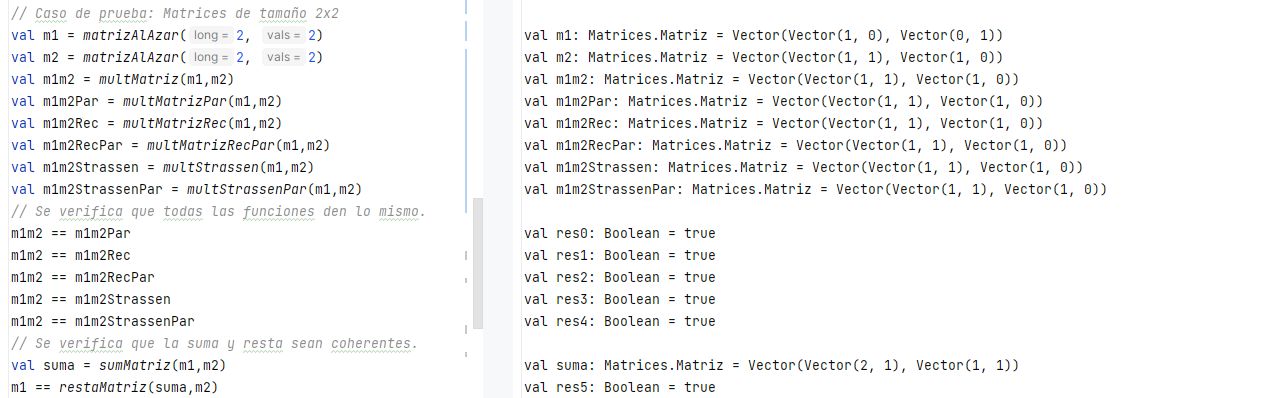
\includegraphics[scale=0.52]{Pruebas1.png}
        \caption{Casos de Prueba matrices de tamaño \(2 \times 2\).}
        \label{1}
    \end{minipage}
\end{figure}

\begin{figure}[h]
    \begin{minipage}{1\textwidth}
        \centering
        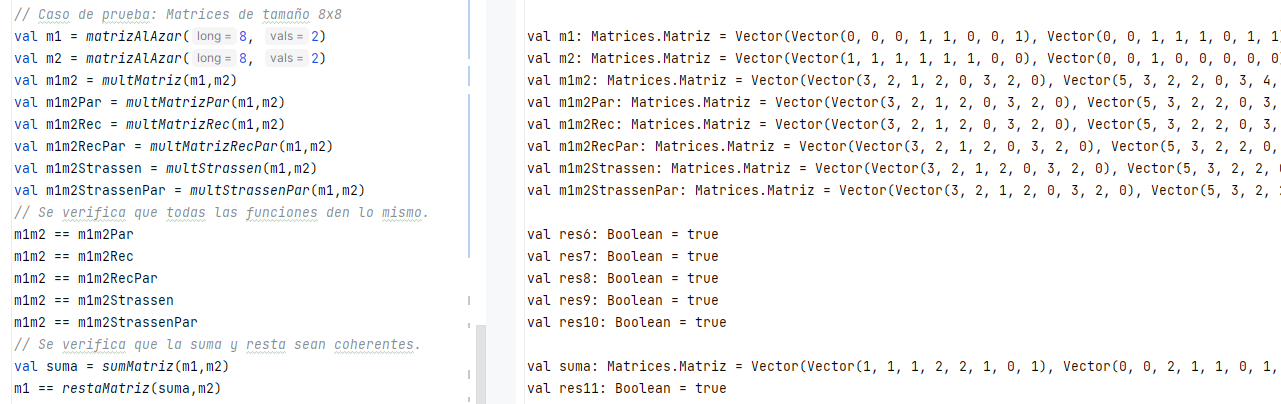
\includegraphics[scale=0.52]{Pruebas2.png}
        \caption{Casos de Prueba matrices de tamaño \(8 \times 8\).}
        \label{1}
    \end{minipage}
\end{figure}

\begin{figure}[h]
    \begin{minipage}{1\textwidth}
        \centering
        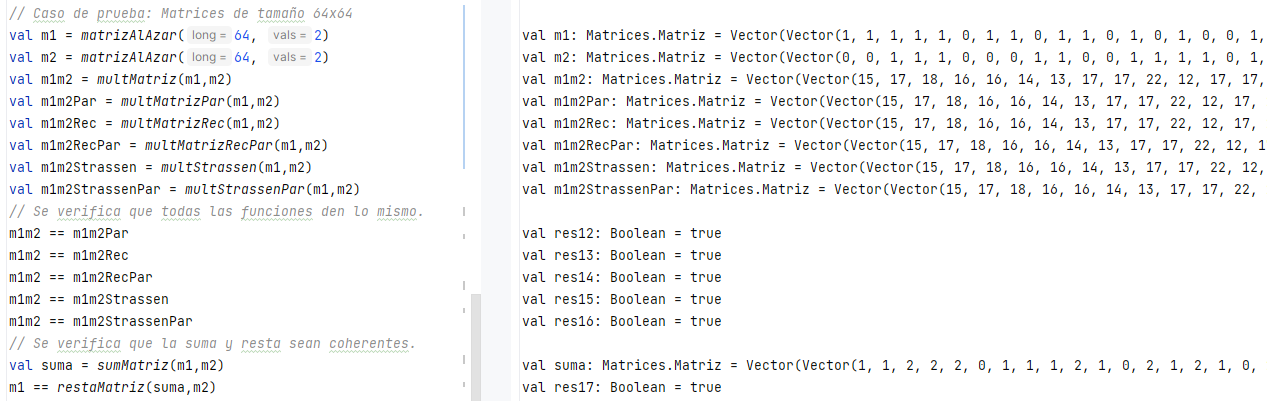
\includegraphics[scale=0.52]{Pruebas3.png}
        \caption{Casos de Prueba matrices de tamaño \(64 \times 64\).}
        \label{1}
    \end{minipage}
\end{figure}

\begin{figure}[h]
    \begin{minipage}{1\textwidth}
        \centering
        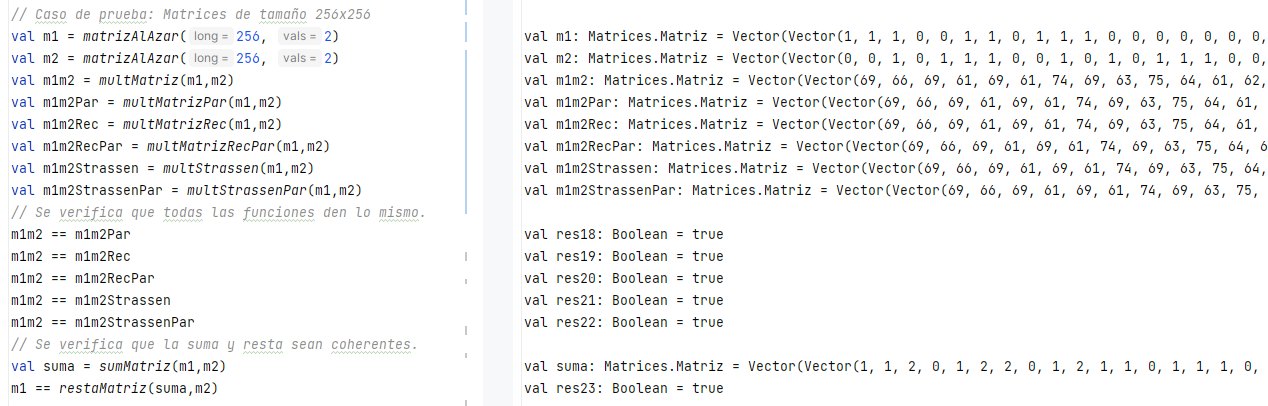
\includegraphics[scale=0.52]{Pruebas4.png}
        \caption{Casos de Prueba matrices de tamaño \(256 \times 256\).}
        \label{1}
    \end{minipage}
\end{figure}

\begin{figure}[h]
    \begin{minipage}{1\textwidth}
        \centering
        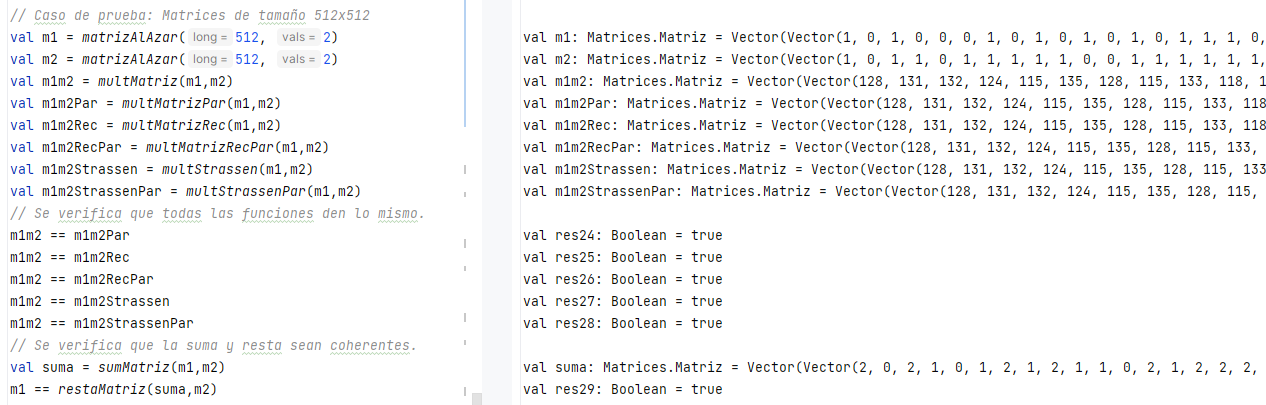
\includegraphics[scale=0.52]{Pruebas5.png}
        \caption{Casos de Prueba matrices de tamaño \(512 \times 512\).}
        \label{1}
    \end{minipage}
\end{figure}

\clearpage 
\section{Informe de desempeño de las funciones secuenciales y de las funciones paralelas}

Claramente, el objetivo de llevar una función cuya ejecución es secuencial a paralelo es el de encontrar una mejora en el rendimiento, o tiempo de ejecución. Se podría afirmar que el objetivo es el de encontrar "aceleración" (en ingles \textit{speedup}), al comparar la versión paralela con su respectiva versión secuencial. Examinemos los resultados entre las versiones paralelas y secuenciales para cada algoritmo de multiplicación. \\

Tal como fue propuesto, se pensó en la implementación de un umbral para las versiones paralelas, el cual se determinó luego de examinar dos ejecuciones de las funciones para los tamaños de matriz: \(2^k \times 2^k\), con \(1 \leq k \leq 8\). Dicho umbral está diseñado para significar el punto, o tamaño de la submatriz entregada en la recursión, tal que, sirva para escoger si se vuelve a ejecutar la versión paralela o se pasa a la versión secuencial. Lo cual permitirá mejor optimización para los casos en que la versión paralela no encuentra mejoría en comparación a la secuencial. Dicho umbral solo fue definido para las versiones recursivas.

\subsection{Algoritmo estándar}

\begin{table}[ht]
\centering
\begin{tabular}{|c|c|c|c|}
\hline
\textbf{Secuencial} & \textbf{Paralelo} & \textbf{Aceleración} & \textbf{Tamaño de Matriz} \\
\hline
0.0441 & 0.3516 & 0.1254 & 2 \\
0.0257 & 0.0805 & 0.3193 & 4 \\
0.0756 & 0.1344 & 0.5625 & 8 \\
0.2811 & 0.9764 & 0.2879 & 16 \\
1.4152 & 0.3435 & 4.1199 & 32 \\
5.3717 & 2.3536 & 2.2823 & 64 \\
37.2918 & 23.6129 & 1.5793 & 128 \\
304.4371 & 171.1787 & 1.7785 & 256 \\
24777.7999 & 1332.7430 & 1.8592 & 512 \\
21777.5295 & 10471.8750 & 2.080 & 1024 \\
\hline
\end{tabular}
\caption{Versión secuencial vs. paralela. Algoritmo estándar. Ejecución No. 1}
\end{table}

\begin{table}[ht]
\centering
\begin{tabular}{|c|c|c|c|}
\hline
\textbf{Secuencial} & \textbf{Paralelo} & \textbf{Aceleración} & \textbf{Tamaño de Matriz} \\
\hline
0.0311 & 0.0647 & 0.4807 & 2 \\
0.0467 & 0.0615 & 0.7593 & 4 \\
0.0524 & 0.2145 & 0.2443 & 8 \\
0.1988 & 0.2128 & 0.9342 & 16 \\
0.7727 & 0.5216 & 1.4814 & 32 \\
5.9568 & 3.2552 & 1.8299 & 64 \\
48.0621 & 28.9965 & 1.6575 & 128 \\
373.5702 & 192.3139 & 1.9425 & 256 \\
2595,4997 & 1328.9630 & 1.9530 & 512 \\
22615.1483 & 10499.465 & 2.1539 & 1024 \\
\hline
\end{tabular}
\caption{Versión secuencial vs. paralela. Algoritmo estándar. Ejecución No. 2}
\end{table}

Examinando los resultados obtenidos, encontramos una clara mejora en el tiempo de ejecución del algoritmo en su versión paralela comparado con su versión secuencial, especialmente en casos donde sus entradas son matrices de tamaño \(32 \times 32\) en adelante.\\

\clearpage

\begin{table}[ht]
\centering
\begin{tabular}{|c|c|c|c|}
\hline
\textbf{Secuencial} & \textbf{Paralelo} & \textbf{Aceleración} & \textbf{Tamaño de Matriz} \\
\hline
0.0775 & 0.1005 & 0.7711 & 2 \\
0.0306 & 0.0617 & 0.4960 & 4 \\
0.0484 & 0.0817 & 0.5924 & 8 \\
0.2144 & 0.2782 & 0.7707 & 16 \\
0.8613 & 0.4970 & 1.7330 & 32 \\
6.1123 & 3.3649 & 1.8165 & 64 \\
45.9702 & 29.1136 & 1.5790 & 128 \\
367.4754 & 201.4365 & 1.8243 & 256 \\
373.5702 & 1256.9938 & 2.0526 & 512 \\
21421.1105 & 10346.4481 & 2.0704 & 1024 \\
\hline
\end{tabular}
\caption{Versión secuencial vs. paralela. Algoritmo estándar. Ejecución No. 3}
\end{table}

\begin{table}[ht]
\centering
\begin{tabular}{|c|c|c|c|}
\hline
\textbf{Secuencial} & \textbf{Paralelo} & \textbf{Aceleración} & \textbf{Tamaño de Matriz} \\
\hline
0.0429 & 0.0791 & 0.5424 & 2 \\
0.0091 & 0.0528 & 0.1723 & 4 \\
0.0368 & 0.0632 & 0.5823 & 8 \\
0.1836 & 0.2955 & 0.6213 & 16 \\
1.2346 & 3.8231 & 0.3229 & 32 \\
6.8564 & 3.1974 & 2.1444 & 64 \\
47.8947 & 26.0675 & 1.8373 & 128 \\
370.4129 & 208.5240 & 1.7764 & 256 \\
2549.8832 & 1336.9112 & 1.9073 & 512 \\
21130.9730 & 10308.4556 & 2.0499 & 1024 \\
\hline
\end{tabular}
\caption{Versión secuencial vs. paralela. Algoritmo estándar. Ejecución No. 4}
\end{table}

\begin{table}[ht]
\centering
\begin{tabular}{|c|c|c|c|}
\hline
\textbf{Secuencial} & \textbf{Paralelo} & \textbf{Aceleración} & \textbf{Tamaño de Matriz} \\
\hline
0.0731 & 0.0833 & 0.8776 & 2 \\
0.0279 & 0.1128 & 0.2473 & 4 \\
0.0940 & 0.1795 & 0.5237 & 8 \\
0.3293 & 1.0097 & 0.3261 & 16 \\
0.6992 & 0.6960 & 1.0046 & 32 \\
4.7594 & 2.4459 & 1.9459 & 64 \\
38.5799 & 20.3091 & 1.8996 & 128 \\
309.1530 & 171.1996 & 1.8058 & 256 \\
2309.3187 & 1150.8890 & 2.0065 & 512 \\
19684.9822 & 10074.0517 & 1.9504 & 1024 \\
\hline
\end{tabular}
\caption{Versión secuencial vs. paralela. Algoritmo estándar. Ejecución No. 5}
\end{table}

Dicho comportamiento es consistente en la mayoría de las ejecuciones en dónde se registraron los datos. alcanzando una aceleración (\textit{speedUp}) promedio entre 1.7324 y 2.0609 (173.2\% a 206.1\%) en los casos evaluados (matrices de tamaño \(32 \times 32\) a \(1024 \times 1024\)). \\

Para los casos en que el tamaño de la matriz cuadrada es menor que 32, se encuentra una pérdida de rendimiento, para lo cual pudo haber sido útil configurar un umbral. Los beneficios de configurar el umbral serán descritos a continuación.

\clearpage

\subsection{Algoritmo recursivo}

Resultados con umbral igual a 2 (que coincide con caso base):

\begin{table}[ht]
\centering
\begin{tabular}{|c|c|c|c|}
\hline
\textbf{Secuencial} & \textbf{Paralelo} & \textbf{Aceleración} & \textbf{Tamaño de Matriz} \\
\hline
0.0125 & 0.0267 & 0.4682 & 2 \\
0.0237 & 0.0626 & 0.3786 & 4 \\
0.1948 & 0.1595 & 1.2213 & 8 \\
0.8592 & 0.4467 & 1.9234 & 16 \\
6.4095 & 2.3477 & 2.7301 & 32 \\
64.4153 & 18.1502 & 3.5490 & 64 \\
431.1129 & 142.2999 & 3.0296 & 128 \\
3465.6238 & 1147.1905 & 3.0210 & 256 \\
27688.8092 & 9288.1190 & 2.9811 & 512 \\
221544.3495 & 74209.6425 & 2.9854 & 1024 \\
\hline
\end{tabular}
\caption{Versión secuencial vs. paralela. Algoritmo recursivo. Ejecución No. 1}
\end{table}

\begin{table}[ht]
\centering
\begin{tabular}{|c|c|c|c|}
\hline
\textbf{Secuencial} & \textbf{Paralelo} & \textbf{Aceleración} & \textbf{Tamaño de Matriz} \\
\hline
0.0028 & 0.0030 & 0.9333 & 2 \\
0.0137 & 0.0471 & 0.2909 & 4 \\
0.1037 & 0.0982 & 1.0560 & 8 \\
0.8597 & 0.4245 & 2.0252 & 16 \\
6.7789 & 2.5174 & 2.6928 & 32 \\
54.2703 & 17.9106 & 3.0301 & 64 \\
431.4056 & 145.1920 & 2.9713 & 128 \\
3466.4742 & 1158.7546 & 2.9916 & 256 \\
27730.1588 & 9362.5781 & 2.9618 & 512 \\
221762.0941 & 74422.2789 & 2.9798 & 1024 \\
\hline
\end{tabular}
\caption{Versión secuencial vs. paralela. Algoritmo recursivo. Ejecución No. 2}
\end{table}

Tal como se puede evidenciar, en las dos primeras ejecuciones registradas, si revizamos el valor de "aceleración" (\textit{speedUp}) hay una clara desaceleración en los casos de matrices de tamaño \(2 \times 2\) y \(4 \times 4\), lo cual significa una pérdida de rendimiento. Por lo cual se configuró un umbral igual a 4, para que desde dicho \textit{punto} se llame a la ejecución en secuencial en vez que al llamado recursivo paralelo.\\

Resultados con umbral igual a 4:

\begin{table}[ht]
\centering
\begin{tabular}{|c|c|c|c|}
\hline
\textbf{Secuencial} & \textbf{Paralelo} & \textbf{Aceleración} & \textbf{Tamaño de Matriz} \\
\hline
0.0145 & 0.0241 & 0.6017 & 2 \\
0.0333 & 0.1421 & 0.2343 & 4 \\
0.1715 & 0.1198 & 1.4316 & 8 \\
0.8637 & 0.3159 & 2.7341 & 16 \\
6.4899 & 2.3561 & 2.7545 & 32 \\
53.5021 & 17.9117 & 2.9870 & 64 \\
441.6521 & 141.4063 & 3.1233 & 128 \\
3425.8259 & 1142.5249 & 2.9985 & 256 \\
27485.6406 & 9121.9758 & 3.0131 & 512 \\
220053.5060 & 72394.4904 & 3.0396 & 1024 \\
\hline
\end{tabular}
\caption{Versión secuencial vs. paralela. Algoritmo recursivo. Ejecución No. 3}
\end{table}

\clearpage

\begin{table}[ht]
\centering
\begin{tabular}{|c|c|c|c|}
\hline
\textbf{Secuencial} & \textbf{Paralelo} & \textbf{Aceleración} & \textbf{Tamaño de Matriz} \\
\hline
0.0019 & 0.0018 & 1.0556 & 2 \\
0.0129 & 0.0128 & 1.0078 & 4 \\
0.1051 & 0.0805 & 1.3056 & 8 \\
0.8377 & 0.3429 & 2.4430 & 16 \\
7.2439 & 2.5745 & 2.8137 & 32 \\
54.3564 & 17.5772 & 3.0924 & 64 \\
430.8232 & 142.7192 & 3.0187 & 128 \\
3455.6864 & 1128.9374 & 3.0610 & 256 \\
27421.6080 & 8961.4008 & 3.0600 & 512 \\
220173.0518 & 72490.5759 & 3.0373 & 1024 \\
\hline
\end{tabular}
\caption{Versión secuencial vs. paralela. Algoritmo recursivo. Ejecución No. 4}
\end{table}

\begin{table}[ht]
\centering
\begin{tabular}{|c|c|c|c|}
\hline
\textbf{Secuencial} & \textbf{Paralelo} & \textbf{Aceleración} & \textbf{Tamaño de Matriz} \\
\hline
0.0354 & 0.0137 & 2.5839 & 2 \\
0.1613 & 0.0844 & 1.9111 & 4 \\
0.5727 & 0.5445 & 1.0518 & 8 \\
1.2409 & 0.6040 & 2.0545 & 16 \\
5.2373 & 2.3092 & 2.2680 & 32 \\
46.2508 & 21.2734 & 2.1741 & 64 \\
382.7379 & 135.1408 & 2.8321 & 128 \\
3081.2330 & 1154.4169 & 2.6691 & 256 \\
24545.3418 & 8863.0016 & 2.7694 & 512 \\
196570.4254 & 71447.9345 & 2.7512 & 1024 \\
\hline
\end{tabular}
\caption{Versión secuencial vs. paralela. Algoritmo de Strassen. Ejecución No. 1}
\end{table}

Tal como era de esperarse, la implementación del umbral sirvió para que para que aquellos casos donde se encontraba pérdida de rendimiento, dejasen de verse afectados en cierta medida (\textit{speedUp} cercano a 1). Lo cual nos permite aceptar a la versión en paralelo, como mejor versión comparada a la secuencial, para todos los casos; alcanzando una mejora en rendimiento en promedio entre: 1.72 y 2.79 (172\% y 279\%), específicamente para los casos donde el tamaño de matriz está entre \(32 \times 32\) a \(256 \times 256\). También cabe reconocerse que la implementación del umbral mejoró el tiempo de ejecución para los casos donde los tamaños de las matrices eran mayores al umbral (\(8 \times 8\) a \(1024 \times 1024\)), pasando de una aceleración de 2.33 a 2.79 en el caso con matrices de tamaño \(1024 \times 1024\).

\clearpage

\subsection{Algoritmo de Strassen}

Resultados con umbral igual a 2 (que coincide con caso base):

\begin{table}[ht]
\centering
\begin{tabular}{|c|c|c|c|}
\hline
\textbf{Secuencial} & \textbf{Paralelo} & \textbf{Aceleración} & \textbf{Tamaño de Matriz} \\
\hline
0.0074 & 0.0062 & 1.1935 & 2 \\
0.0497 & 0.0978 & 0.5082 & 4 \\
0.4916 & 0.2135 & 2.3026 & 8 \\
1.5815 & 0.6785 & 2.3309 & 16 \\
7.4228 & 3.7767 & 1.9654 & 32 \\
43.0942 & 16.0412 & 2.6865 & 64 \\
310.8794 & 104.7491 & 2.9678 & 128 \\
2180.7757 & 721.7616 & 3.0215 & 256 \\
15267.6590 & 5081.7448 & 3.0044 & 512 \\
107643.8453 & 35968.0719 & 2.9928 & 1024 \\
\hline
\end{tabular}
\caption{Versión secuencial vs. paralela. Algoritmo de Strassen. Ejecución No. 1}
\end{table}

\begin{table}[ht]
\centering
\begin{tabular}{|c|c|c|c|}
\hline
\textbf{Secuencial} & \textbf{Paralelo} & \textbf{Aceleración} & \textbf{Tamaño de Matriz} \\
\hline
0.0031 & 0.0019 & 1.6316 & 2 \\
0.0157 & 0.0555 & 0.2829 & 4 \\
0.1135 & 0.1508 & 0.7527 & 8 \\
0.8633 & 0.5423 & 1.5919 & 16 \\
32.1531 & 2.3563 & 13.6456 & 32 \\
45.5246 & 15.4341 & 2.9496 & 64 \\
309.4869 & 105.5268 & 2.9328 & 128 \\
2171.0991 & 733.3728 & 2.9604 & 256 \\
15310.5616 & 4964.9316 & 3.0837 & 512 \\
107246.9233 & 35804.7617 & 2.9953 & 1024 \\
\hline
\end{tabular}
\caption{Versión secuencial vs. paralela. Algoritmo de Strassen. Ejecución No. 2}
\end{table}

Examinando los resultados de las dos primeras ejecuciones, encontramos la necesidad de configurar el umbral igual a 4, tal como en el algoritmo recursivo. Lo cual, ayudaría a mejorar el desempeño en los casos con matrices de tamaños 2 y 4. Donde habría una mejoría del rendimiento, haciéndola cercana a un \textit{speedUp} de valor 1, equivalente al rendimiento de la versión en secuencial. Por supuesto, debe verificarse esto en los resultados.\\

Resultados con umbral igual a 4:

\begin{table}[ht]
\centering
\begin{tabular}{|c|c|c|c|}
\hline
\textbf{Secuencial} & \textbf{Paralelo} & \textbf{Aceleración} & \textbf{Tamaño de Matriz} \\
\hline
0.0132 & 0.0192 & 0.6875 & 2 \\
0.0455 & 0.0711 & 0.6399 & 4 \\
0.2121 & 0.1659 & 1.2785 & 8 \\
1.0221 & 0.4563 & 2.2400 & 16 \\
7.4084 & 2.4072 & 3.0776 & 32 \\
44.5917 & 14.9022 & 2.9923 & 64 \\
312.1107 & 103.7498 & 3.0083 & 128 \\
2188.5974 & 727.9144 & 3.0067 & 256 \\
15365.3213 & 5027.4427 & 3.0563 & 512 \\
107400.5579 & 35167.8846 & 3.0539 & 1024 \\
\hline
\end{tabular}
\caption{Versión secuencial vs. paralela. Algoritmo de Strassen. Ejecución No. 3}
\end{table}

\begin{table}[ht]
\centering
\begin{tabular}{|c|c|c|c|}
\hline
\textbf{Secuencial} & \textbf{Paralelo} & \textbf{Aceleración} & \textbf{Tamaño de Matriz} \\
\hline
0.0025 & 0.0025 & 1.0000 & 2 \\
0.0165 & 0.0161 & 1.0248 & 4 \\
0.1202 & 0.1200 & 1.0017 & 8 \\
0.8457 & 0.3752 & 2.2540 & 16 \\
6.4712 & 2.5333 & 2.5545 & 32 \\
43.7750 & 15.1152 & 2.8961 & 64 \\
307.6558 & 104.3044 & 2.9496 & 128 \\
2129.5280 & 714.8112 & 2.9791 & 256 \\
15431.3588 & 5037.5490 & 3.0633 & 512 \\
108309.4602 & 35638.6469 & 3.0391 & 1024 \\
\hline
\end{tabular}
\caption{Versión secuencial vs. paralela. Algoritmo de Strassen. Ejecución No. 4}
\end{table}

\begin{table}[ht]
\centering
\begin{tabular}{|c|c|c|c|}
\hline
\textbf{Secuencial} & \textbf{Paralelo} & \textbf{Aceleración} & \textbf{Tamaño de Matriz} \\
\hline
0.0026 & 0.0021 & 1.2381 & 2 \\
0.0165 & 0.0151 & 1.0927 & 4 \\
0.1178 & 0.0861 & 1.3682 & 8 \\
0.8503 & 0.4506 & 1.8870 & 16 \\
6.5147 & 2.3431 & 2.7804 & 32 \\
41.5459 & 16.1500 & 2.5725 & 64 \\
307.2176 & 102.9226 & 2.9849 & 128 \\
2463.2580 & 723.8962 & 3.4028 & 256 \\
15378.5597 & 5023.8190 & 3.0611 & 512 \\
108069.4118 & 35076.7282 & 3.0809 & 1024 \\
\hline
\end{tabular}
\caption{Versión secuencial vs. paralela. Algoritmo de Strassen. Ejecución No. 5}
\end{table}


Luego de configurar el umbral pudo identificarse una mejor estabilidad en el rendimiento para los casos mencionados (alcanzando y manteniendo un \textit{speedUp} cercano 1).

Tal como era de esperarse, se encontró una mejora en el rendimiento al pasar de la versión secuencial a la paralela, obteniendo una mejora en rendimiento promedio entre: 2.13 y 3.06 (mejoras entre un 113\% a 206\% más de rendimiento). Lo cual se puede encontrar similar a la mejora encontrada en el algoritmo recursivo.\\

Sin embargo recordemos que estas comparaciones son entre versiones secuencial y paralela de cada algoritmo. Por lo cual, aún no podemos inferir cuál algoritmo resultó ser el mejor de todos.

\clearpage

\section{Análisis comparativo de las diferentes soluciones}

A continuación estudiaremos los diferentes algoritmos de multiplicación de matrices, comparándolos en términos de su rendimiento, en función del tamaño de matriz las matrices cuadradas de entrada. \\

Anteriormente, comparamos en cada algoritmo sus versiones secuencial y paralela, y encontramos que hubo mejora en el rendimiento; liderando siempre las versiones paralelas. Sin embargo, aún nos queda examinar si el haber implementado un algoritmo u otro habrá valido la pena, en términos de mejora en rendimiento. Así mismo, verificar, en el caso en que no hubo mejora en rendimiento, si las versiones paralelas lograron esa mejora en rendimiento esperada comparadas al algoritmo estándar.\\

Lograremos identificar cuál de los algoritmos implementados resulta ser el más rápido. De qué depende que la aceleración sea mejor. Y de sobre en qué casos es mejor usar la versión secuencial/paralela de cada algoritmo de multiplicación de matrices.\\

Comparemos, primero las versiones secuenciales.

\subsection{Versiones secuenciales}

\subsubsection{Algoritmo estándar contra algoritmo recursivo}

\begin{table}[ht]
\centering
\begin{tabular}{|c|c|c|c|}
\hline
\textbf{Estándar} & \textbf{Recursivo} & \textbf{Aceleración} & \textbf{Tamaño de Matriz} \\
\hline
0.0441 & 0.0125 & 3.528 & 2 \\
0.0257 & 0.0237 & 1.0844 & 4 \\
0.0756 & 0.1948 & 0.3881 & 8 \\
0.2811 & 0.8592 & 0.3272 & 16 \\
1.4152 & 6.4095 & 0.2208 & 32 \\
5.3717 & 64.4153 & 0.0834 & 64 \\
37.2918 & 431.1129 & 0.0865 & 128 \\
304.4371 & 3465.6238 & 0.0878 & 256 \\
2477.7999 & 27688.8092 & 0.0895 & 512 \\
21777.5295 & 221544.3495 & 0.0983 & 1024 \\
\hline
\end{tabular}
\caption{Algoritmo estándar vs. recursivo. Versión secuencial. Ejecución No. 1}
\end{table}

\begin{table}[ht]
\centering
\begin{tabular}{|c|c|c|c|}
\hline
\textbf{Estándar} & \textbf{Recursivo} & \textbf{Aceleración} & \textbf{Tamaño de Matriz} \\
\hline
0.0311 & 0.0028 & 11.1071 & 2 \\
0.0467 & 0.0137 & 3.4088 & 4 \\
0.0524 & 0.1037 & 0.5053 & 8 \\
0.1988 & 0.8597 & 0.2312 & 16 \\
0.7727 & 6.7789 & 0.1140 & 32 \\
5.9568 & 54.2703 & 0.1098 & 64 \\
48.0621 & 431.4056 & 0.1114 & 128 \\
373.5702 & 3466.4742 & 0.1078 & 256 \\
2595.4997 & 27730.1588 & 0.0936 & 512 \\
22615.1483 & 221762.0941 & 0.1020 & 1024 \\
\hline
\end{tabular}
\caption{Algoritmo estándar vs. recursivo. Versión secuencial. Ejecución No. 2}
\end{table}

\begin{table}[ht]
\centering
\begin{tabular}{|c|c|c|c|}
\hline
\textbf{Estándar} & \textbf{Recursivo} & \textbf{Aceleración} & \textbf{Tamaño de Matriz} \\
\hline
0.0775 & 0.0145 & 5.3448 & 2 \\
0.0306 & 0.0333 & 0.9189 & 4 \\
0.0484 & 0.1715 & 0.2822 & 8 \\
0.2144 & 0.8637 & 0.2482 & 16 \\
0.8613 & 6.4899 & 0.1327 & 32 \\
6.1123 & 53.5021 & 0.1142 & 64 \\
45.9702 & 441.6521 & 0.1041 & 128 \\
367.4754 & 3425.8259 & 0.1073 & 256 \\
2580.1542 & 27485.6406 & 0.0939 & 512 \\
21421.1105 & 220053.506 & 0.0973 & 1024 \\
\hline
\end{tabular}
\caption{Algoritmo estándar vs. recursivo. Versión secuencial. Ejecución No. 3}
\end{table}

\begin{table}[ht]
\centering
\begin{tabular}{|c|c|c|c|}
\hline
\textbf{Estándar} & \textbf{Recursivo} & \textbf{Aceleración} & \textbf{Tamaño de Matriz} \\
\hline
0.0429 & 0.0019 & 22.5789 & 2 \\
0.0091 & 0.0129 & 0.7054 & 4 \\
0.0368 & 0.1051 & 0.3501 & 8 \\
0.1836 & 0.8377 & 0.2192 & 16 \\
1.2346 & 7.2439 & 0.1704 & 32 \\
6.8564 & 54.3564 & 0.1261 & 64 \\
47.8947 & 430.8232 & 0.1112 & 128 \\
370.4129 & 3455.6864 & 0.1072 & 256 \\
2549.8832 & 27421.608 & 0.0930 & 512 \\
21130.973 & 220173.0518 & 0.0960 & 1024 \\
\hline
\end{tabular}
\caption{Algoritmo estándar vs. recursivo. Versión secuencial. Ejecución No. 4}
\end{table}

\begin{table}[ht]
\centering
\begin{tabular}{|c|c|c|c|}
\hline
\textbf{Estándar} & \textbf{Recursivo} & \textbf{Aceleración} & \textbf{Tamaño de Matriz} \\
\hline
0.0731 & 0.0354 & 2.0650 & 2 \\
0.0279 & 0.1613 & 0.1730 & 4 \\
0.0940 & 0.5727 & 0.1641 & 8 \\
0.3293 & 1.2409 & 0.2654 & 16 \\
0.6992 & 5.2373 & 0.1335 & 32 \\
4.7594 & 46.2508 & 0.1029 & 64 \\
38.5799 & 382.7379 & 0.1008 & 128 \\
309.1530 & 3081.2330 & 0.1003 & 256 \\
2309.3187 & 24545.3418 & 0.0941 & 512 \\
19648.9822 & 196570.4254 & 0.1000 & 1024 \\
\hline
\end{tabular}
\caption{Algoritmo estándar vs. recursivo. Versión secuencial. Ejecución No. 5}
\end{table}

\clearpage

Tal como se puede evidenciar en las tablas 16 y 17, no se encuentra mejora de rendimiento al pasar del algoritmo estándar al recursivo. Es más, entre más grande es el tamaño de las matrices el valor de \textit{speedUp} tiende a nivelarse cerca a 0.10. Lo mismo ocurrió en las 5 ejecuciones registradas.\\

Lo anterior pudo darse debido a la cantidad de operaciones encontradas en el algoritmo recursivo, que aunque podría considerarse de menor complejidad, significaría una mayor cantidad de memoria requerida, y recordemos que el acceso a memoria no es tan rápido como las operaciones del procesador. \\ 

Quizá deba estudiarse el rendimiento de los operadores ++, .\textit{zip} y .\textit{map} usados en la reconstrucción de las matrices a retornar.\\

Examinemos si lo mismo pasó entre el algoritmo recursivo y el de Strassen.\\

\subsubsection{Algoritmo recursivo contra algoritmo de Strassen}

\begin{table}[ht]
\centering
\begin{tabular}{|c|c|c|c|}
\hline
\textbf{Recursivo} & \textbf{Strassen} & \textbf{Aceleración} & \textbf{Tamaño de Matriz} \\
\hline
0.0125 & 0.0074 & 1.6892 & 2 \\
0.0237 & 0.0497 & 0.4769 & 4 \\
0.1948 & 0.4916 & 0.3963 & 8 \\
0.8592 & 1.5815 & 0.5433 & 16 \\
6.4095 & 7.4228 & 0.8635 & 32 \\
64.4153 & 43.0942 & 1.4948 & 64 \\
431.1129 & 310.8794 & 1.3868 & 128 \\
3465.6238 & 2180.7757 & 1.5892 & 256 \\
27688.8092 & 15267.659 & 1.8136 & 512 \\
221544.3495 & 107643.8453 & 2.0581 & 1024 \\
\hline
\end{tabular}
\caption{Algoritmo recursivo vs. Strassen. Versión secuencial. Ejecución No. 1}
\end{table}

\begin{table}[ht]
\centering
\begin{tabular}{|c|c|c|c|}
\hline
\textbf{Recursivo} & \textbf{Strassen} & \textbf{Aceleración} & \textbf{Tamaño de Matriz} \\
\hline
0.0028 & 0.0031 & 0.9032 & 2 \\
0.0137 & 0.0157 & 0.8726 & 4 \\
0.1037 & 0.1135 & 0.9137 & 8 \\
0.8597 & 0.8633 & 0.9958 & 16 \\
6.7789 & 32.1531 & 0.2108 & 32 \\
54.2703 & 45.5246 & 1.1921 & 64 \\
431.4056 & 309.4869 & 1.3939 & 128 \\
3466.4742 & 2171.0991 & 1.5966 & 256 \\
27730.1588 & 15310.5616 & 1.8112 & 512 \\
221762.0941 & 107246.9233 & 2.0678 & 1024 \\
\hline
\end{tabular}
\caption{Algoritmo recursivo vs. Strassen. Versión secuencial. Ejecución No. 2}
\end{table}

\begin{table}[ht]
\centering
\begin{tabular}{|c|c|c|c|}
\hline
\textbf{Recursivo} & \textbf{Strassen} & \textbf{Aceleración} & \textbf{Tamaño de Matriz} \\
\hline
0.0145 & 0.0132 & 1.0985 & 2 \\
0.0333 & 0.0455 & 0.7319 & 4 \\
0.1715 & 0.2121 & 0.8086 & 8 \\
0.8637 & 1.0221 & 0.8450 & 16 \\
6.4899 & 7.4084 & 0.8760 & 32 \\
53.5021 & 44.5917 & 1.1998 & 64 \\
441.6521 & 312.1107 & 1.4150 & 128 \\
3425.8259 & 2188.5974 & 1.5653 & 256 \\
27485.6406 & 15365.3213 & 1.7888 & 512 \\
220053.506 & 107400.5579 & 2.0489 & 1024 \\
\hline
\end{tabular}
\caption{Algoritmo recursivo vs. Strassen. Versión secuencial. Ejecución No. 3}
\end{table}

\begin{table}[ht]
\centering
\begin{tabular}{|c|c|c|c|}
\hline
\textbf{Recursivo} & \textbf{Strassen} & \textbf{Aceleración} & \textbf{Tamaño de Matriz} \\
\hline
0.0019 & 0.0025 & 0.76 & 2 \\
0.0129 & 0.0165 & 0.7818 & 4 \\
0.1051 & 0.1202 & 0.8744 & 8 \\
0.8377 & 0.8457 & 0.9905 & 16 \\
7.2439 & 6.4712 & 1.1194 & 32 \\
54.3564 & 43.7750 & 1.2417 & 64 \\
430.8232 & 307.6558 & 1.4003 & 128 \\
3455.6864 & 2129.5280 & 1.6227 & 256 \\
27421.608 & 15431.3588 & 1.7770 & 512 \\
220173.0518 & 108309.4602 & 2.0328 & 1024 \\
\hline
\end{tabular}
\caption{Algoritmo recursivo vs. Strassen. Versión secuencial. Ejecución No. 4}
\end{table}

\begin{table}[ht]
\centering
\begin{tabular}{|c|c|c|c|}
\hline
\textbf{Recursivo} & \textbf{Strassen} & \textbf{Aceleración} & \textbf{Tamaño de Matriz} \\
\hline
0.0354 & 0.0026 & 13.6154 & 2 \\
0.1613 & 0.0165 & 9.7758 & 4 \\
0.5727 & 0.1178 & 4.8616 & 8 \\
1.2409 & 0.8503 & 1.4594 & 16 \\
5.2373 & 6.5147 & 0.8039 & 32 \\
46.2508 & 41.5459 & 1.1132 & 64 \\
382.7379 & 307.2176 & 1.2458 & 128 \\
3081.2330 & 2463.2580 & 1.2509 & 256 \\
24545.3418 & 15378.5597 & 1.5961 & 512 \\
196570.4254 & 108069.4118 & 1.8189 & 1024 \\
\hline
\end{tabular}
\caption{Algoritmo recursivo vs. Strassen. Versión secuencial. Ejecución No. 5}
\end{table}


Es evidente que entre algoritmos recursivos (recordemos la naturaleza recursiva del algoritmo de Strassen) sí se encuentra una mejoría en el rendimiento. Una mejoría que va entre el 20\% y 95\% más de rendimiento (especialmente entre los casos de matrices de tamaños \(64 \times 64\) en adelante). La disminución del número de multiplicaciones recursivas, logró aportar mayor aceleración comparado al algoritmo recursivo.\\

\clearpage

\subsubsection{Algoritmo estándar contra algoritmo de Strassen}

\begin{table}[ht]
\centering
\begin{tabular}{|c|c|c|c|}
\hline
\textbf{Estándar} & \textbf{Strassen} & \textbf{Aceleración} & \textbf{Tamaño de Matriz} \\
\hline
0.0441 & 0.0074 & 5.9595 & 2 \\
0.0257 & 0.0497 & 0.5171 & 4 \\
0.0756 & 0.4916 & 0.1538 & 8 \\
0.2811 & 1.5815 & 0.1777 & 16 \\
1.4152 & 7.4228 & 0.1907 & 32 \\
5.3717 & 43.0942 & 0.1247 & 64 \\
37.2918 & 310.8794 & 0.1200 & 128 \\
304.4371 & 2180.7757 & 0.1396 & 256 \\
2477.7999 & 15267.659 & 0.1623 & 512 \\
21777.5295 & 107643.8453 & 0.2023 & 1024 \\
\hline
\end{tabular}
\caption{Algoritmo estándar vs. Strassen. Versión secuencial. Ejecución No. 1}
\end{table}


\begin{table}[ht]
\centering
\begin{tabular}{|c|c|c|c|}
\hline
\textbf{Estándar} & \textbf{Strassen} & \textbf{Aceleración} & \textbf{Tamaño de Matriz} \\
\hline
0.0311 & 0.0031 & 10.0323 & 2 \\
0.0467 & 0.0157 & 2.9745 & 4 \\
0.0524 & 0.1135 & 0.4617 & 8 \\
0.1988 & 0.8633 & 0.2303 & 16 \\
0.7727 & 32.1531 & 0.0240 & 32 \\
5.9568 & 45.5246 & 0.1308 & 64 \\
48.0621 & 309.4869 & 0.1553 & 128 \\
373.5702 & 2171.0991 & 0.1721 & 256 \\
2595.4997 & 15310.5616 & 0.1695 & 512 \\
22615.1483 & 107246.9233 & 0.2109 & 1024 \\
\hline
\end{tabular}
\caption{Algoritmo estándar vs. Strassen. Versión secuencial. Ejecución No. 2}
\end{table}

\begin{table}[ht]
\centering
\begin{tabular}{|c|c|c|c|}
\hline
\textbf{Estándar} & \textbf{Strassen} & \textbf{Aceleración} & \textbf{Tamaño de Matriz} \\
\hline
0.0775 & 0.0132 & 5.8712 & 2 \\
0.0306 & 0.0455 & 0.6725 & 4 \\
0.0484 & 0.2121 & 0.2282 & 8 \\
0.2144 & 1.0221 & 0.2098 & 16 \\
0.8613 & 7.4084 & 0.1163 & 32 \\
6.1123 & 44.5917 & 0.1371 & 64 \\
45.9702 & 312.1107 & 0.1473 & 128 \\
367.4754 & 2188.5974 & 0.1679 & 256 \\
2580.1542 & 15365.3213 & 0.1679 & 512 \\
21421.1105 & 107400.5579 & 0.1995 & 1024 \\
\hline
\end{tabular}
\caption{Algoritmo estándar vs. Strassen. Versión secuencial. Ejecución No. 3}
\end{table}

\clearpage

\begin{table}[ht]
\centering
\begin{tabular}{|c|c|c|c|}
\hline
\textbf{Estándar} & \textbf{Strassen} & \textbf{Aceleración} & \textbf{Tamaño de Matriz} \\
\hline
0.0429 & 0.0025 & 17.16 & 2 \\
0.0091 & 0.0165 & 0.5515 & 4 \\
0.0368 & 0.1202 & 0.3062 & 8 \\
0.1836 & 0.8457 & 0.2171 & 16 \\
1.2346 & 6.4712 & 0.1908 & 32 \\
6.8564 & 43.7750 & 0.1566 & 64 \\
47.8947 & 307.6558 & 0.1557 & 128 \\
370.4129 & 2129.5280 & 0.1739 & 256 \\
2549.8832 & 15431.3588 & 0.1652 & 512 \\
21130.9730 & 108309.4602 & 0.1951 & 1024 \\
\hline
\end{tabular}
\caption{Algoritmo estándar vs. Strassen. Versión secuencial. Ejecución No. 4}
\end{table}

\begin{table}[ht]
\centering
\begin{tabular}{|c|c|c|c|}
\hline
\textbf{Estándar} & \textbf{Strassen} & \textbf{Aceleración} & \textbf{Tamaño de Matriz} \\
\hline
0.0731 & 0.0026 & 28.1154 & 2 \\
0.0279 & 0.0165 & 1.6909 & 4 \\
0.0940 & 0.1178 & 0.7980 & 8 \\
0.3293 & 0.8503 & 0.3873 & 16 \\
0.6992 & 6.5147 & 0.1073 & 32 \\
4.7594 & 41.5459 & 0.1146 & 64 \\
38.5799 & 307.2176 & 0.1256 & 128 \\
309.1530 & 2463.2580 & 0.1255 & 256 \\
2309.3187 & 15378.5597 & 0.1502 & 512 \\
19648.9822 & 108069.4118 & 0.1818 & 1024 \\
\hline
\end{tabular}
\caption{Algoritmo estándar vs. Strassen. Versión secuencial. Ejecución No. 5}
\end{table}


Es claro observar que la mejora en rendimiento del algoritmo de Strassen contra el Recursivo está reflejada en su relación con el estándar, donde podemos identificar un valor de \textit{speedUp} que tiende cerca a 0.20 para matrices de mayor tamaño. Lo que sí resulta algo fuera de lo esperado es que el rendimiento del algoritmo de Strassen no superó el rendimiento del algoritmo estándar en los tamaños de matriz estudiados, lo cual es algo fuera de lo esperado, ya que en teoría el algoritmo de Strassen es el más rápido, pero que resultó quedar en segundo lugar, detrás del algoritmo estándar. Verifiquemos si para las versiones paralelas ocurrió lo mismo.

\subsection{Versiones paralelas}

\subsubsection{Algoritmo estándar contra algoritmo recursivo}

\begin{table}[ht]
\centering
\begin{tabular}{|c|c|c|c|}
\hline
\textbf{Estándar} & \textbf{Recursivo} & \textbf{Aceleración} & \textbf{Tamaño de Matriz} \\
\hline
0.3516 & 0.0267 & 13.1685 & 2 \\
0.0805 & 0.0626 & 1.2859 & 4 \\
0.1344 & 0.1595 & 0.8426 & 8 \\
0.9764 & 0.4467 & 2.1858 & 16 \\
0.3435 & 2.3477 & 0.1463 & 32 \\
2.3536 & 18.1502 & 0.1297 & 64 \\
23.6129 & 142.2999 & 0.1659 & 128 \\
171.1787 & 1147.1905 & 0.1492 & 256 \\
1332.7430 & 9288.1190 & 0.1435 & 512 \\
10471.8750 & 74209.6425 & 0.1411 & 1024 \\
\hline
\end{tabular}
\caption{Algoritmo estándar vs. recursivo. Versión paralela. Ejecución No. 1}
\end{table}

\begin{table}[ht]
\centering
\begin{tabular}{|c|c|c|c|}
\hline
\textbf{Estándar} & \textbf{Recursivo} & \textbf{Aceleración} & \textbf{Tamaño de Matriz} \\
\hline
0.0647 & 0.0030 & 21.5667 & 2 \\
0.0615 & 0.0471 & 1.3057 & 4 \\
0.2145 & 0.0982 & 2.1843 & 8 \\
0.2128 & 0.4245 & 0.5013 & 16 \\
0.5216 & 2.5174 & 0.2072 & 32 \\
3.2552 & 17.9106 & 0.1817 & 64 \\
28.9965 & 145.1920 & 0.1997 & 128 \\
192.3139 & 1158.7546 & 0.1660 & 256 \\
1328.9630 & 9362.5781 & 0.1419 & 512 \\
10499.4650 & 74422.2789 & 0.1411 & 1024 \\
\hline
\end{tabular}
\caption{Algoritmo estándar vs. recursivo. Versión paralela. Ejecución No. 2}
\end{table}

\begin{table}[ht]
\centering
\begin{tabular}{|c|c|c|c|}
\hline
\textbf{Estándar} & \textbf{Recursivo} & \textbf{Aceleración} & \textbf{Tamaño de Matriz} \\
\hline
0.1005 & 0.0241 & 4.1701 & 2 \\
0.0617 & 0.1421 & 0.4342 & 4 \\
0.0817 & 0.1198 & 0.6820 & 8 \\
0.2782 & 0.3159 & 0.8807 & 16 \\
0.4970 & 2.3561 & 0.2109 & 32 \\
3.3649 & 17.9117 & 0.1879 & 64 \\
29.1136 & 141.4063 & 0.2059 & 128 \\
201.4365 & 1142.5249 & 0.1763 & 256 \\
1256.9938 & 9121.9758 & 0.1378 & 512 \\
10346.4481 & 72394.4904 & 0.1429 & 1024 \\
\hline
\end{tabular}
\caption{Algoritmo estándar vs. recursivo. Versión paralela. Ejecución No. 3}
\end{table}

\begin{table}[ht]
\centering
\begin{tabular}{|c|c|c|c|}
\hline
\textbf{Estándar} & \textbf{Recursivo} & \textbf{Aceleración} & \textbf{Tamaño de Matriz} \\
\hline
0.0791 & 0.0018 & 43.9444 & 2 \\
0.0528 & 0.0128 & 4.1250 & 4 \\
0.0632 & 0.0805 & 0.7851 & 8 \\
0.2955 & 0.3429 & 0.8618 & 16 \\
3.8231 & 2.5745 & 1.4850 & 32 \\
3.1974 & 17.5772 & 0.1819 & 64 \\
26.0675 & 142.7192 & 0.1826 & 128 \\
208.5240 & 1128.9374 & 0.1847 & 256 \\
1336.9112 & 8961.4008 & 0.1492 & 512 \\
10308.4556 & 72490.5759 & 0.1422 & 1024 \\
\hline
\end{tabular}
\caption{Algoritmo estándar vs. recursivo. Versión paralela. Ejecución No. 4}
\end{table}

\begin{table}[ht]
\centering
\begin{tabular}{|c|c|c|c|}
\hline
\textbf{Estándar} & \textbf{Recursivo} & \textbf{Aceleración} & \textbf{Tamaño de Matriz} \\
\hline
0.0833 & 0.0137 & 6.0803 & 2 \\
0.1128 & 0.0844 & 1.3365 & 4 \\
0.1795 & 0.5445 & 0.3297 & 8 \\
1.0097 & 0.6040 & 1.6717 & 16 \\
0.6960 & 2.3092 & 0.3014 & 32 \\
2.4459 & 21.2734 & 0.1150 & 64 \\
20.3091 & 135.1408 & 0.1503 & 128 \\
171.1996 & 1154.4169 & 0.1483 & 256 \\
1150.8890 & 8863.0016 & 0.1299 & 512 \\
10074.0517 & 71447.9345 & 0.1410 & 1024 \\
\hline
\end{tabular}
\caption{Algoritmo estándar vs. recursivo. Versión paralela. Ejecución No. 5}
\end{table}

\clearpage

\subsubsection{Algoritmo recursivo contra algoritmo de Strassen}

\begin{table}[ht]
\centering
\begin{tabular}{|c|c|c|c|}
\hline
\textbf{Recursivo} & \textbf{Strassen} & \textbf{Aceleración} & \textbf{Tamaño de Matriz} \\
\hline
0.0267 & 0.0062 & 4.3065 & 2 \\
0.0626 & 0.0978 & 0.6401 & 4 \\
0.1595 & 0.2135 & 0.7471 & 8 \\
0.4467 & 0.6785 & 0.6584 & 16 \\
2.3477 & 3.7767 & 0.6216 & 32 \\
18.1502 & 16.0412 & 1.1315 & 64 \\
142.2999 & 104.7491 & 1.3585 & 128 \\
1147.1905 & 721.7616 & 1.5894 & 256 \\
9288.1190 & 5081.7448 & 1.8277 & 512 \\
74209.6425 & 35968.0719 & 2.0632 & 1024 \\
\hline
\end{tabular}
\caption{Algoritmo recursivo vs. Strassen. Versión paralela. Ejecución No. 1}
\end{table}

\begin{table}[ht]
\centering
\begin{tabular}{|c|c|c|c|}
\hline
\textbf{Recursivo} & \textbf{Strassen} & \textbf{Aceleración} & \textbf{Tamaño de Matriz} \\
\hline
0.0030 & 0.0019 & 1.5790 & 2 \\
0.0471 & 0.0555 & 0.8486 & 4 \\
0.0982 & 0.1508 & 0.6512 & 8 \\
0.4245 & 0.5423 & 0.7828 & 16 \\
2.5174 & 2.3563 & 1.0684 & 32 \\
17.9106 & 15.4341 & 1.1605 & 64 \\
145.1920 & 105.5268 & 1.3759 & 128 \\
1158.7546 & 733.3728 & 1.5800 & 256 \\
9362.5781 & 4964.9316 & 1.8857 & 512 \\
74422.2789 & 35804.7617 & 2.0786 & 1024 \\
\hline
\end{tabular}
\caption{Algoritmo recursivo vs. Strassen. Versión paralela. Ejecución No. 2}
\end{table}

\begin{table}[ht]
\centering
\begin{tabular}{|c|c|c|c|}
\hline
\textbf{Recursivo} & \textbf{Strassen} & \textbf{Aceleración} & \textbf{Tamaño de Matriz} \\
\hline
0.0241 & 0.0192 & 1.2552 & 2 \\
0.1421 & 0.0711 & 1.9986 & 4 \\
0.1198 & 0.1659 & 0.7221 & 8 \\
0.3159 & 0.4563 & 0.6923 & 16 \\
2.3561 & 2.4072 & 0.9788 & 32 \\
17.9117 & 14.9022 & 1.2019 & 64 \\
141.4063 & 103.7498 & 1.3630 & 128 \\
1142.5249 & 727.9144 & 1.5696 & 256 \\
9121.9758 & 5027.4427 & 1.8144 & 512 \\
72394.4904 & 35167.8846 & 2.0585 & 1024 \\
\hline
\end{tabular}
\caption{Algoritmo recursivo vs. Strassen. Versión paralela. Ejecución No. 3}
\end{table}

\begin{table}[ht]
\centering
\begin{tabular}{|c|c|c|c|}
\hline
\textbf{Recursivo} & \textbf{Strassen} & \textbf{Aceleración} & \textbf{Tamaño de Matriz} \\
\hline
0.0018 & 0.0025 & 0.7200 & 2 \\
0.0128 & 0.0161 & 0.7950 & 4 \\
0.0805 & 0.1200 & 0.6708 & 8 \\
0.3429 & 0.3752 & 0.9139 & 16 \\
2.5745 & 2.5333 & 1.0163 & 32 \\
17.5772 & 15.1152 & 1.1629 & 64 \\
142.7192 & 104.3044 & 1.3683 & 128 \\
1128.9374 & 714.8112 & 1.5794 & 256 \\
8961.4008 & 5037.5490 & 1.7789 & 512 \\
72490.5759 & 35638.6469 & 2.0340 & 1024 \\
\hline
\end{tabular}
\caption{Algoritmo recursivo vs. Strassen. Versión paralela. Ejecución No. 4}
\end{table}

\begin{table}[ht]
\centering
\begin{tabular}{|c|c|c|c|}
\hline
\textbf{Recursivo} & \textbf{Strassen} & \textbf{Aceleración} & \textbf{Tamaño de Matriz} \\
\hline
0.0137 & 0.0021 & 6.5238 & 2 \\
0.0844 & 0.0151 & 5.5894 & 4 \\
0.5445 & 0.0861 & 6.3240 & 8 \\
0.6040 & 0.4506 & 1.3404 & 16 \\
2.3092 & 2.3431 & 0.9855 & 32 \\
21.2734 & 16.1500 & 1.3172 & 64 \\
135.1408 & 102.9226 & 1.3130 & 128 \\
1154.4169 & 723.8962 & 1.5947 & 256 \\
8863.0016 & 5023.8190 & 1.7642 & 512 \\
71447.9345 & 35076.7282 & 2.0369 & 1024 \\
\hline
\end{tabular}
\caption{Algoritmo recursivo vs. Strassen. Versión paralela. Ejecución No. 5}
\end{table}

\clearpage

\subsubsection{Algoritmo estándar contra algoritmo de Strassen}

\begin{table}[ht]
\centering
\begin{tabular}{|c|c|c|c|}
\hline
\textbf{Estándar} & \textbf{Strassen} & \textbf{Aceleración} & \textbf{Tamaño de Matriz} \\
\hline
0.3516 & 0.0062 & 56.7097 & 2 \\
0.0805 & 0.0978 & 0.8231 & 4 \\
0.1344 & 0.2135 & 0.6295 & 8 \\
0.9764 & 0.6785 & 1.4391 & 16 \\
0.3435 & 3.7767 & 0.0910 & 32 \\
2.3536 & 16.0412 & 0.1467 & 64 \\
23.6129 & 104.7491 & 0.2254 & 128 \\
171.1787 & 721.7616 & 0.2372 & 256 \\
1332.7430 & 5081.7448 & 0.2623 & 512 \\
10471.8750 & 35968.0719 & 0.2911 & 1024 \\
\hline
\end{tabular}
\caption{Algoritmo estándar vs. Strassen. Versión paralela. Ejecución No. 1}
\end{table}

\begin{table}[ht]
\centering
\begin{tabular}{|c|c|c|c|}
\hline
\textbf{Estándar} & \textbf{Strassen} & \textbf{Aceleración} & \textbf{Tamaño de Matriz} \\
\hline
0.0647 & 0.0019 & 34.0526 & 2 \\
0.0615 & 0.0555 & 1.1081 & 4 \\
0.2145 & 0.1508 & 1.4224 & 8 \\
0.2128 & 0.5423 & 0.3924 & 16 \\
0.5216 & 2.3563 & 0.2214 & 32 \\
3.2552 & 15.4341 & 0.2109 & 64 \\
28.9965 & 105.5268 & 0.2748 & 128 \\
192.3139 & 733.3728 & 0.2622 & 256 \\
1328.9630 & 4964.9316 & 0.2677 & 512 \\
10499.4650 & 35804.7617 & 0.2932 & 1024 \\
\hline
\end{tabular}
\caption{Algoritmo estándar vs. Strassen. Versión paralela. Ejecución No. 2}
\end{table}

\begin{table}[ht]
\centering
\begin{tabular}{|c|c|c|c|}
\hline
\textbf{Estándar} & \textbf{Strassen} & \textbf{Aceleración} & \textbf{Tamaño de Matriz} \\
\hline
0.1005 & 0.0192 & 5.2344 & 2 \\
0.0617 & 0.0711 & 0.8678 & 4 \\
0.0817 & 0.1659 & 0.4925 & 8 \\
0.2782 & 0.4563 & 0.6097 & 16 \\
0.4970 & 2.4072 & 0.2065 & 32 \\
3.3649 & 14.9022 & 0.2258 & 64 \\
29.1136 & 103.7498 & 0.2806 & 128 \\
201.4365 & 727.9144 & 0.2767 & 256 \\
1256.9938 & 5027.4427 & 0.2500 & 512 \\
10346.4481 & 35167.8846 & 0.2942 & 1024 \\
\hline
\end{tabular}
\caption{Algoritmo estándar vs. Strassen. Versión paralela. Ejecución No. 3}
\end{table}

\begin{table}[ht]
\centering
\begin{tabular}{|c|c|c|c|}
\hline
\textbf{Estándar} & \textbf{Strassen} & \textbf{Aceleración} & \textbf{Tamaño de Matriz} \\
\hline
0.0791 & 0.0025 & 31.6400 & 2 \\
0.0528 & 0.0161 & 3.2795 & 4 \\
0.0632 & 0.1200 & 0.5267 & 8 \\
0.2955 & 0.3752 & 0.7876 & 16 \\
3.8231 & 2.5333 & 1.5091 & 32 \\
3.1974 & 15.1152 & 0.2115 & 64 \\
26.0675 & 104.3044 & 0.2499 & 128 \\
208.5240 & 714.8112 & 0.2917 & 256 \\
1336.9112 & 5037.5490 & 0.2654 & 512 \\
10308.4556 & 35638.6469 & 0.2892 & 1024 \\
\hline
\end{tabular}
\caption{Algoritmo estándar vs. Strassen. Versión paralela. Ejecución No. 4}
\end{table}

\begin{table}[ht]
\centering
\begin{tabular}{|c|c|c|c|}
\hline
\textbf{Estándar} & \textbf{Strassen} & \textbf{Aceleración} & \textbf{Tamaño de Matriz} \\
\hline
0.0833 & 0.0021 & 39.6667 & 2 \\
0.1128 & 0.0151 & 7.4702 & 4 \\
0.1795 & 0.0861 & 2.0848 & 8 \\
1.0097 & 0.4506 & 2.2408 & 16 \\
0.6960 & 2.3431 & 0.2970 & 32 \\
2.4459 & 16.1500 & 0.1514 & 64 \\
20.3091 & 102.9226 & 0.1973 & 128 \\
171.1996 & 723.8962 & 0.2365 & 256 \\
1150.8890 & 5023.8190 & 0.2291 & 512 \\
10074.0517 & 35076.7282 & 0.2872 & 1024 \\
\hline
\end{tabular}
\caption{Algoritmo estándar vs. Strassen. Versión paralela. Ejecución No. 5}
\end{table}


Basta con examinar de manera global los resultados encontrados al comparar las versiones paralelas de los algoritmos, que no se alejan demasiado de los resultados obtenidos para las implementaciones secuenciales (manteniéndose la misma relación entre el algoritmo de Strassen con el Recursivo). Sí es interesante, encontrar que tampoco en las versiones paralelas se consiguió superar el rendimiento del algoritmo estándar en paralelo, el cual depende plenamente del rendimiento del método \(Vector.tabulate\), aunque algo mejorado debido a que se generan las dos "mitades" de la matriz a la vez.

Por lo que nos permite pensar que los métodos sobre colecciones en la librería estándar de Scala están muy bien optimizados, donde ni el enfoque de dividir y conquistar logra superar dicha optimización. De hecho, hubo optimizaciones que se intentaron. Antes se habían implementado las versiones paralelas con \textit{parallel} y no se obtuvieron resultados óptimos, sobre todo para los casos de matrices de gran tamaño (desde 1024). por ello se usó \(task\) para buscar llevar a cabo todas las recursiones en simultaneo, en los algoritmos recursivos.\\

Lo anterior nos permite cuestionar si nuestras implementaciones recursivas paralelas fueron fructíferas. En términos de superar a la implementación estándar, podría llegarse a decir que no, sin embargo, es claro que sí lograron superar en rendimiento a sus respectivas implementaciones en secuencial. Por lo que nos permite confiar y afirmar que sí se alcanzó el objetivo de mejorar el rendimiento mediante paralelismo y concurrencia.\\

Y, para responder de manera directa a la pregunta sobre en qué casos es mejor la versión secuencial sobre la versión paralela, recordemos lo comentado acerca de la configuración del umbral en las implementaciones en paralelo, basada en las dos ejecuciones iniciales. Con ello en cuenta, podemos decir que justo en los casos donde las matrices tenían un tamaño menor o igual al valor del umbral sugerido (casos donde el \textit{speedUp} era menor que 1; el umbral antes de ser configurado era igual a 2) para cada algoritmo en paralelo, era mejor la versión en secuencial comparada a la paralela. Sin embargo, configurar el umbral a este nuevo valor respectivo, llevó a minimizar la desventaja de los algoritmos en paralelo comparados con los secuenciales en dichos casos. i.e. tal como se comentó anteriormente, tanto para el algoritmo \textit{recursivo} como para el de \textit{Strassen} los casos donde las matrices tenían tamaño menor o igual a \(4 \times 4\) se encontraba un \textit{speedUp} menor que 1, indicando una clara desaceleración, permitiendo afirmar que para dichos casos era mejor el algoritmo secuencial. Pero dicho efecto se contrarrestó (niveló) luego de configurar el umbral a 4.

\clearpage

\section{Implementando el producto punto usando paralelismo de datos} 

Por último estudiaremos el beneficio de hacer uso de paralelismo de datos mediante la evaluación comparativa entre las funciones: \(prodPunto()\) y \(prodPuntoParD()\). Para extraer el rendimiento y \(speedUp\) al comparar ambas funciones se hará uso de la función provista en el paquete \(Benchmark\): compararProdPunto.\\

Examinemos los resultados para vectores de tamaño dado en potencias de 2.

\begin{table}[ht]
\centering
\begin{tabular}{|c|c|c|c|}
\hline
\textbf{prodPunto} & \textbf{prodPuntoParD} & \textbf{Speedup} & \textbf{Tamaño} \\
\hline
0.0086 & 0.2152 & 0.03996 & 2 \\
0.0157 & 0.3819 & 0.04111 & 16 \\
0.0035 & 0.4753 & 0.00736 & 32 \\
0.0078 & 0.4812 & 0.01621 & 128 \\
0.0158 & 0.4567 & 0.03460 & 256 \\
0.0303 & 0.2646 & 0.11451 & 1024 \\
0.0961 & 0.2179 & 0.44103 & 2048 \\
0.1435 & 0.3231 & 0.44413 & 4096 \\
0.2398 & 0.3035 & 0.79012 & 8192 \\
0.4365 & 0.3651 & 1.19556 & 16384 \\
0.8402 & 0.5145 & 1.63304 & 32768 \\
1.5303 & 0.8174 & 1.87216 & 65536 \\
\hline
\end{tabular}
\caption{Resultados benchmark \textit{prodPunto}() vs. \textit{prodPuntoParD}(). Ejecución seleccionada 1}
\end{table}

\begin{table}[ht]
\centering
\begin{tabular}{|c|c|c|c|}
\hline
\textbf{prodPunto (s)} & \textbf{prodPuntoParD (s)} & \textbf{Speedup} & \textbf{Tamaño} \\
\hline
0.0084 & 0.2096 & 0.04008 & 2 \\
0.0029 & 0.3550 & 0.00817 & 16 \\
0.0066 & 0.3944 & 0.01673 & 32 \\
0.0078 & 0.5324 & 0.01465 & 128 \\
0.0101 & 0.4553 & 0.02218 & 256 \\
0.0294 & 0.4393 & 0.06692 & 1024 \\
0.0938 & 0.2324 & 0.40361 & 2048 \\
0.1449 & 0.3137 & 0.46191 & 4096 \\
0.2370 & 0.2594 & 0.91365 & 8192 \\
0.4346 & 0.3156 & 1.37706 & 16384 \\
0.8173 & 0.6119 & 1.33568 & 32768 \\
1.5581 & 0.8365 & 1.86264 & 65536 \\
\hline
\end{tabular}
\caption{Resultados benchmark \textit{prodPunto}() vs. \textit{prodPuntoParD}(). Ejecución seleccionada 2}
\end{table}

Como podemos evidenciar, examinando la tabla anterior, el uso de \textit{prodPuntoParD}() sería viable, en comparación dcon su versión secuencial, cuando los tamaños de los vectores sean del orden de \(2^{14} = 16384\) en adelante. Por lo cual no nos hubiese ayudado en la ejecución de los casos propuestos de multiplicación de matrices. Una multiplicación matricial de dicho tamaño tomaría muchas horas, aún con la paralelización aplicada. Sin embargo, si la intención o diseño de las funciones para operar matrices es de multiplicar matrices de tamaño mayor o igual que \(16384 \time 16384\), la paralelización de datos sí podría comenzar a brindar beneficios. Por que estamos hablando de un incremento del rendimiento mayor al 25\% aproximadamente, y aún más si se consideran vectores de tamaño más grande (superando el 80\% en los casos estudiados), tal como se puede ver en los resultados obtenidos.\\

Por lo tanto, la paralelización de datos claro que brinda beneficios, siempre y cuando se requieran operar matrices o vectores lo suficientemente grandes. Pero no sería beneficiosa para los casos propuestos anteriormente. Usamos matrices de tamaño máximo de \(1024 \times 1024\), para lo cual hubiera significado en una pérdida del rendimiento de más del 70\% en las operaciones de producto punto, las cuales son clave para la multiplicación de matrices.

\clearpage
\end{document}